\newcommand{\X}{\mathbf{X}}
\section{Method}\label{s:method}

\begin{figure}
\centering
%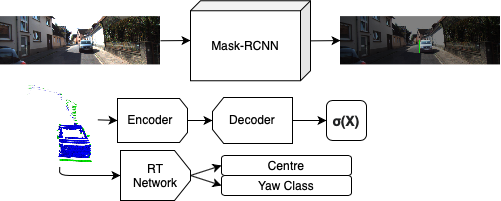
\includegraphics[width=0.75\textwidth]{figures/method/FPN.png}
\includegraphics[width=1.0\textwidth]{figures/system.pdf}
\caption{Network architecture. Dashed arrows in red show the flow of the gradients during the backward pass. Alignment loss is evaluated for each yaw bin $\theta_k$ and the optimal yaw is used to supervise the yaw classification network $\Phi_r$ (see sec.~\ref{s:direct-yaw}).}\label{fig:network_architecture}
% source: system.svg created in Inkscape
% https://drive.google.com/file/d/1hjJ9znYa3mIgfydyCUSzDMKnB1lmoKT3/view?usp=sharing
\end{figure}

Our goal is to estimate the 3D bounding box of objects given as input videos with 2D mask predictions and LiDAR point clouds.
We discuss first how this problem can be approached by direct fitting and then develop a much better learning-based solution.

\subsection{Shape model fitting}\label{s:shapemodel}

We first describe how a 3D bounding box can be fitted to the available data in a direct manner.
To this end, let $I \in \mathbb{R}^{3\times H\times W}$ be a RGB image obtained from the camera sensor and let $L \subset\mathbb{R}^3$ be a corresponding finite collection of 3D points $\X\in L$ extracted from the LiDAR sensor.
Furthermore, let $m \in \{0,1\}^{H \times W}$ be the 2D mask of the object obtained from a system such as Mask R-CNN~\cite{he17mask} from image $I$.
Our goal is to convert the 2D mask $m$ into a corresponding 3D bounding box $B$.

To do so, assume that the LiDAR points are expressed in the reference frame of the camera and that the camera calibration function $k : \mathbb{R}^2 \rightarrow \Omega = \{1,\dots,H\}\times\{1,\dots,W\}$ is known.
The calibration function is defined such that the 3D point $\X=(X,Y,Z)$ projects onto the image pixel $u = k(\pi(\X))$ where $\pi(X,Y,Z)=(X/Z,Y/Z)$ is the perspective projection.
In particular, the subset of LiDAR points $L_m \subset L$ that project onto the 2D mask $m$ is given by:
$
L_m
=
L \cap
(k \circ \pi)^*(m)
$
where ${}^*$ denotes the pre-image of a function.
In practice, this is a crude filtering step, because the masks are imprecise and not perfectly aligned to the LiDAR and because LiDAR may sometimes see `through' the object, for instance in correspondence of glass surfaces
% as one point of the mask $m$ in the pixel space obviously potentially corresponds to an infinite number of 3D LiDAR points; this property manifests in practice by including 3D LiDAR points which are in front of the vehicle as well as LiDAR points behind the actual object, as for example car windows are transparent to LiDAR
(see \cref{fig:dataset_example}).

\begin{figure}
    \centering
    \begin{tabular}{c c c c}
         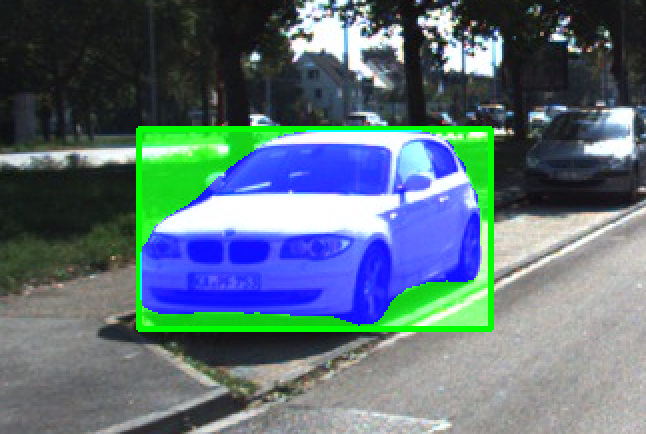
\includegraphics[width=0.25\textwidth]{figures/method/examples/rgb-2.png}
        &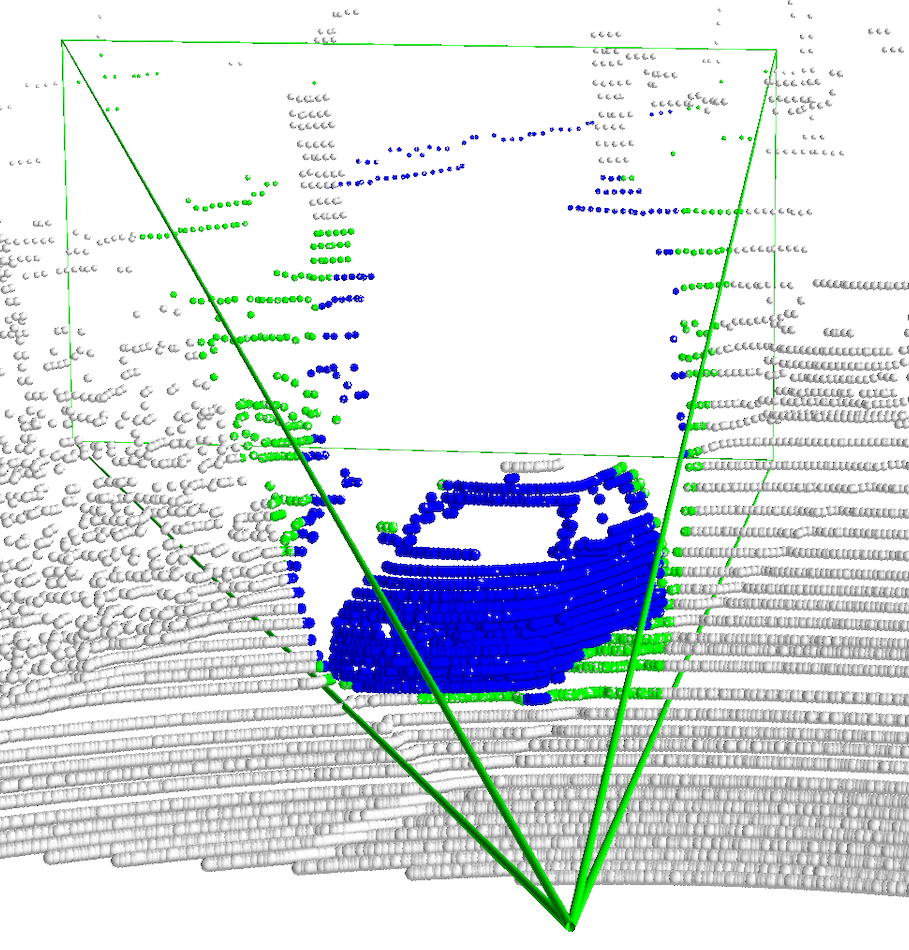
\includegraphics[width=0.2\textwidth]{figures/method/examples/pcd-2.png} &
         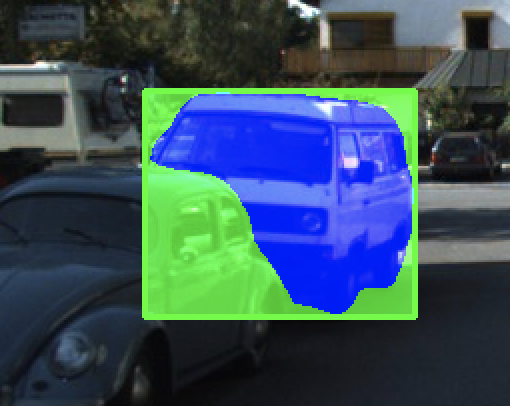
\includegraphics[width=0.2\textwidth]{figures/method/examples/rgb-4.png}
        &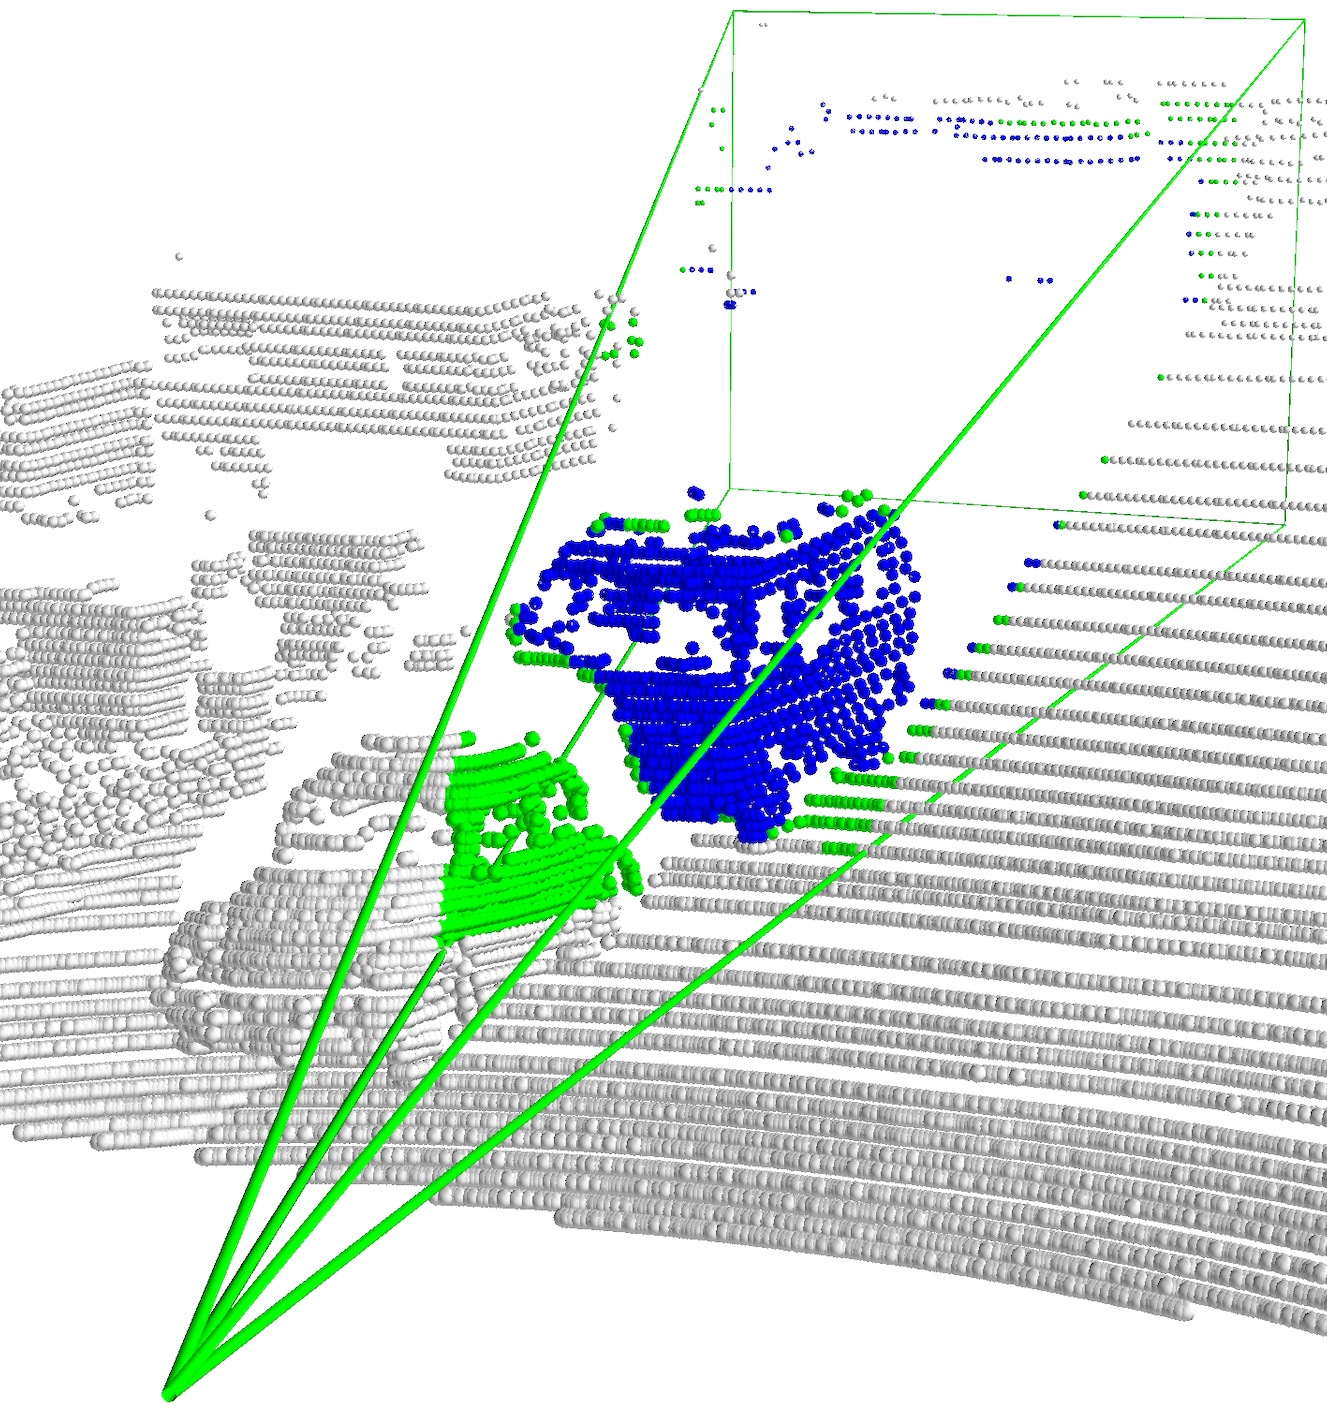
\includegraphics[width=0.2\textwidth]{figures/method/examples/pcd-4.png} \\
    \end{tabular}
    \caption{
    For each pair, left: RGB input image with Mask R-CNN predicted box and highlighted pixels inside the mask.
    Right: LiDAR points in blue represent those inside the 2D mask, green those outside.
    Note that, while the image mask removes many outliers, not all of them ares.}\label{fig:dataset_example}
\end{figure}


In order to fit a 3D bounding box $B$ to $L_m$, we use a weak prior on the 3D shape of the object.
Specifically, we assume that a 3D template surface $S_0\subset\mathbb{R}^3$ is available, for example as simplicial (triangulated) mesh.
We fit the 3D surface to the LiDAR points by considering a rigid motion $g \in SE(3)$ which, applied to $S_0$, results in the posed mesh
$
S = gS_0 = \{g\X : \X \in S_0\}.
$
We then define a distance between the mesh and the 3D LiDAR points as follows:
\begin{align}\label{e:dist1}
d(S|L_m)
&=
\frac{1}{|L_m|}
\sum_{\X \in L_m}
\min_{\X' \in S}
\|\X' - \X \|^2.
\end{align}
This quantity is similar to a Chamfer distance, but it only considers half of it:
this is because most of the 3D points that belong to the template object are \emph{not} be visible in a given view (in particular, at least half are self-occluded), so not all points in the template mesh have a corresponding LiDAR point.

% While~\cref{e:dist1} can be computed exactly if $S$ is a mesh, in practice we found it beneficial to replace this quantity with the following `noisy estimate':
% \begin{align}\label{e:dist2}
%   \hat d(S|L_m)
%   &=
%   E_{\hat S}\left[
%   \frac{1}{|L_m|}
%   \sum_{\X \in L_m}
%   \min_{\X' \in \hat S}
%   \|\X' - \X \|^2
%   \right]
% \end{align}
% where $\hat S$ is a finite collection of 3D points sampled uniformly at random on the surface $S$ of the object (in the experiment, we set $|\hat S| = 1000$).
% In addition to making the calculation of~\cref{e:dist1} faster, using \cref{e:dist2} in a stochastic optimizer might help convergence by escaping local optima.

Given a 2D object mask $m$ and its corresponding LiDAR points $L_m$, we can find the pose $g$ of the object by minimizing $d(g S_0|L_m)$ with respect to $g \in SE(3)$.
Then the bounding box of the object $m$ is given by $gB_0$ where $B_0 \subset \mathbb{R}^3$ is the 3D bounding box that tightly encloses the template $S_0$.

In accordance with prior work~\cite{geiger12are-we-ready,qin20weakly,meng2020ws3d}, we can in practice carry out the minimization not over the of full space $SE(3)$, but only on 4-DoF transformation $g = [R_\theta,~\mathbf{T}]$ where the rotation $R_\theta$ is restricted to the \emph{yaw} $\theta$ (rotation perpendicular to the ground plane).
Even so, direct minimization of~\cref{e:dist1} is in practice prone to failure because individual partial LiDAR point clouds do not contain sufficient information and fitting results are thus ambiguous (we do not report results in this setting as they are extremely poor).

%\subsection{Learning-based fitting}\label{s:model}

% Because directly fitting~\cref{e:dist2} to a small set of LiDAR points that only observe a fraction of the surface $S_0$ is ambiguous and works poorly due to noise and occlusions ({\color{red} see ablation experiment}),

Our solution to the ambiguity of fitting~\cref{e:dist1} is to \emph{share information} across all object instances in the dataset.
We do this by training a deep neural network
$
\Phi : \operatorname{Fin}(\mathbb{R}^3) \rightarrow SE(3)
$
mapping the LiDAR points $L_m$ to the corresponding object pose $g = \Phi(L_m)$ directly.
The network $\Phi$ can be trained in a self-supervised manner by minimizing \cref{e:dist1} averaged over the entire dataset
$
\mathcal{D}
$
as
\begin{align}\label{e:simpleloss}
  %  (R_m, \mathbf{T}_m) &= \Phi(L_m) \\\label{e:simpleloss}
  \mathcal{L}(\Phi|\mathcal{D})
  &=
  \frac{1}{|\mathcal{D}|}
  \sum_{(L_m,m)\in\mathcal{D}}
  d(g_m S_0 | L_{m}),
  ~~~
  \text{where} ~ g_m = \Phi(L_m).
\end{align}
%{\color{red}Note that our goal is not so much to train the predictor $\Phi$ (although this is also useful), but rather to obtain the fits $g_m=[R_{\theta_m}~ \mathbf{T}_m] = \Phi(L_m)$.}
% The network is an auxiliary byproduct of this process.
% In particular, note that we retain the output of the network on the dataset $\mathcal{D}$ (which would normally be discarded as this is also the training set) -- this is a form of self-supervision.

\subsection{Modelling and discounting outliers}

% \begin{figure}
    \centering
    \begin{tabular}{c c c c}

        %  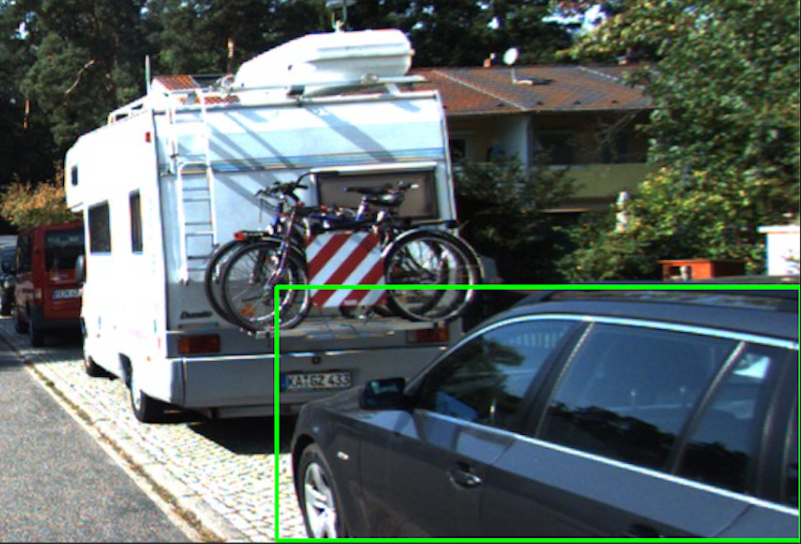
\includegraphics[width=0.2\textwidth]{figures/method/ambiguous/ex2/rgb.png}
        % &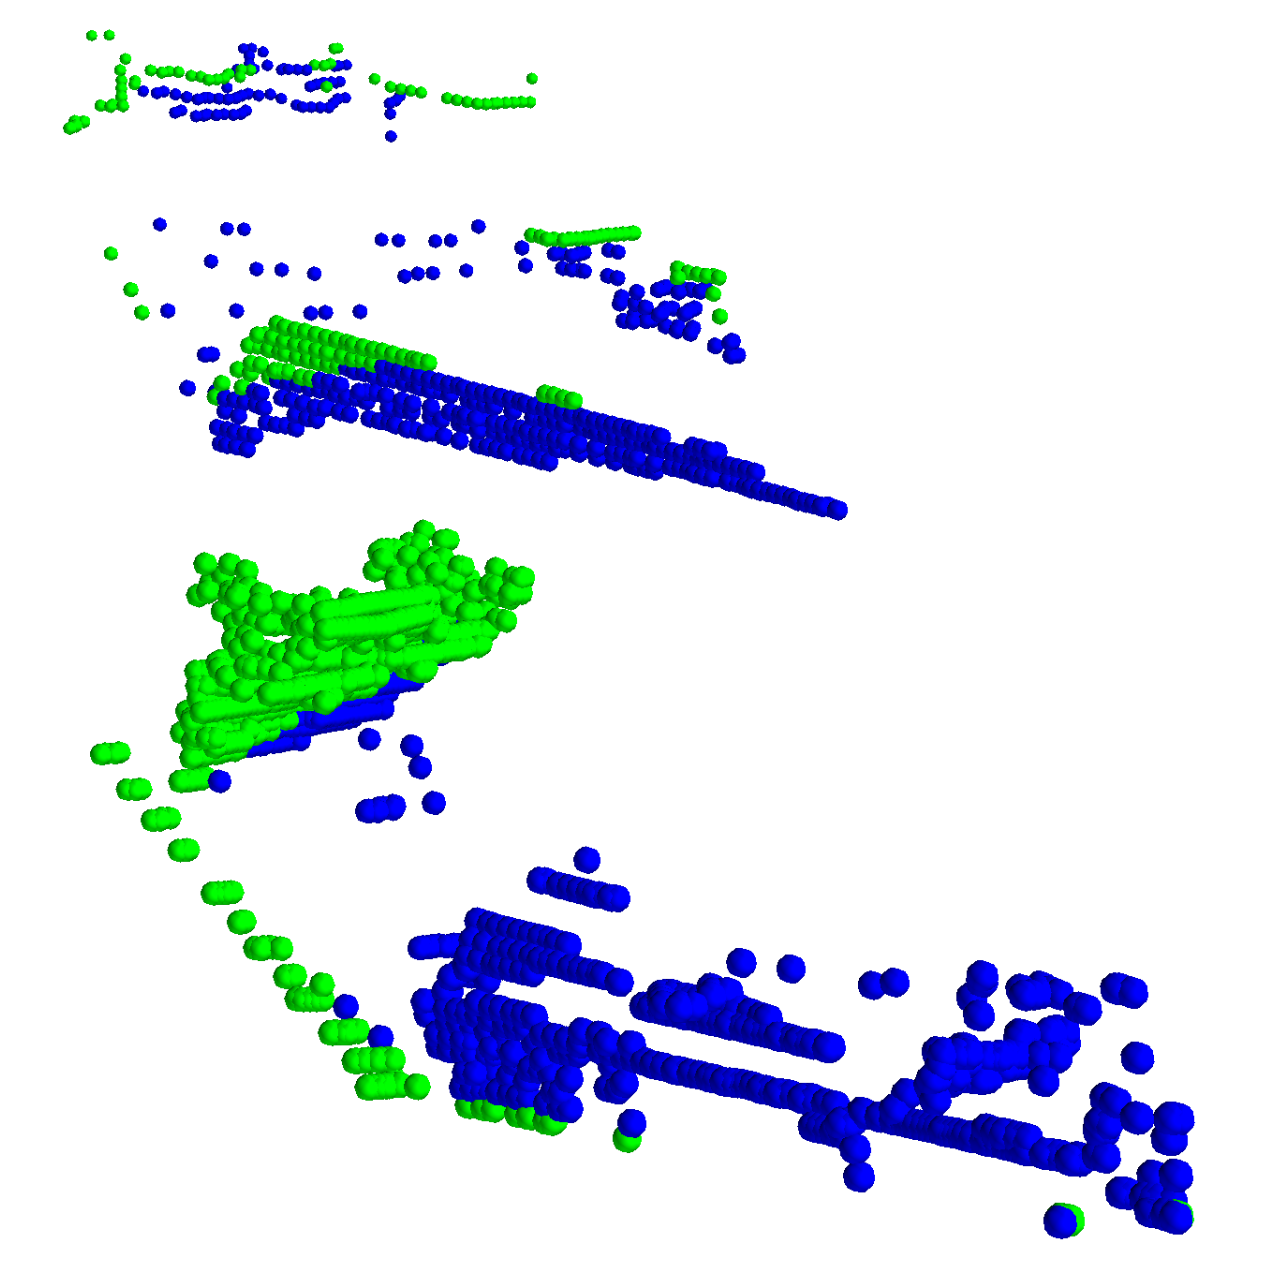
\includegraphics[width=0.2\textwidth]{figures/method/ambiguous/ex2/pcd.png} &
         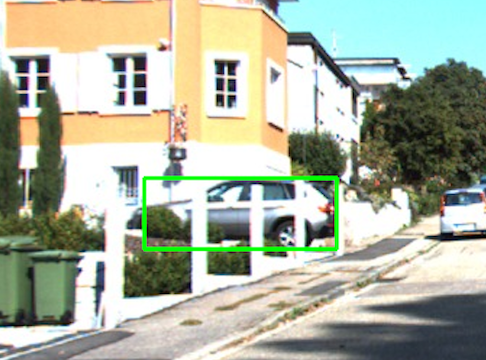
\includegraphics[width=0.2\textwidth]{figures/method/ambiguous/ex3/rgb.png}
        &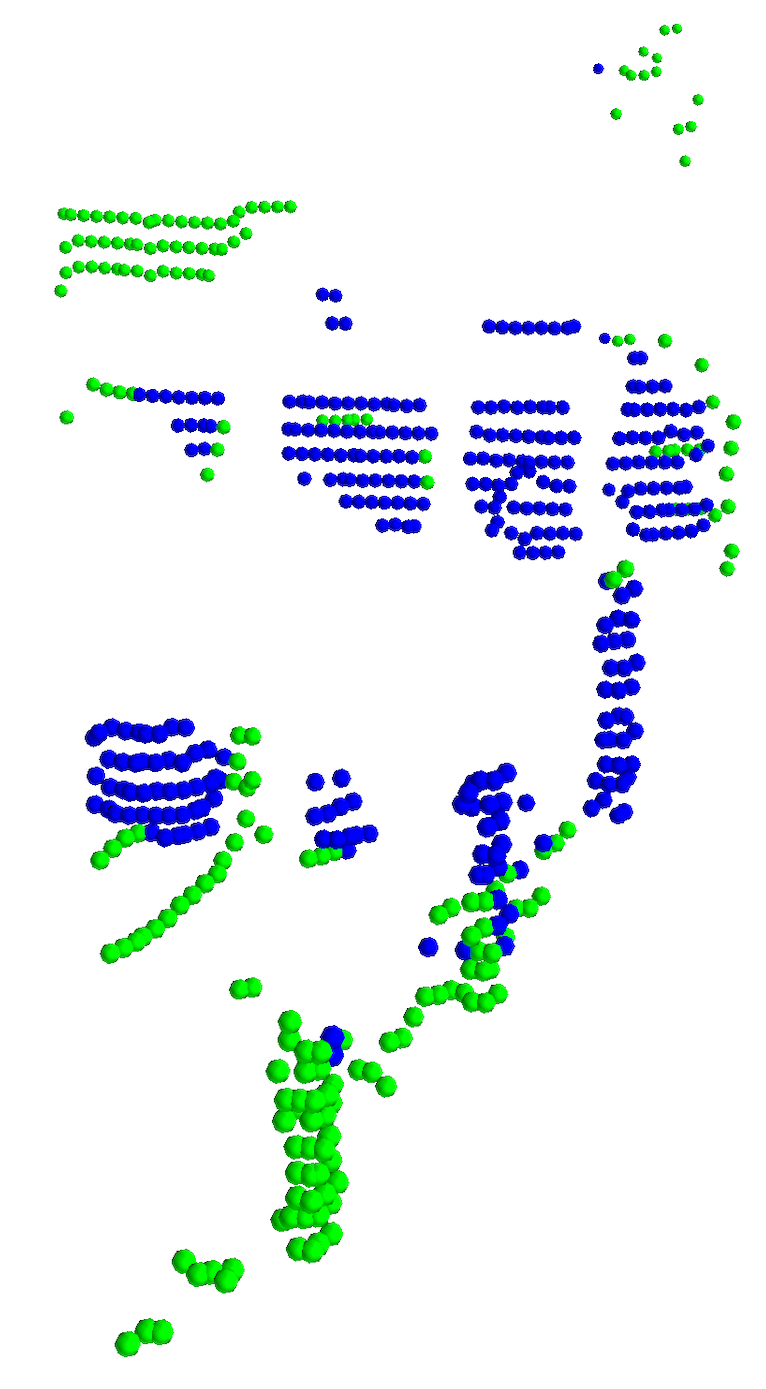
\includegraphics[width=0.1\textwidth]{figures/method/ambiguous/ex3/pcd.png} &
         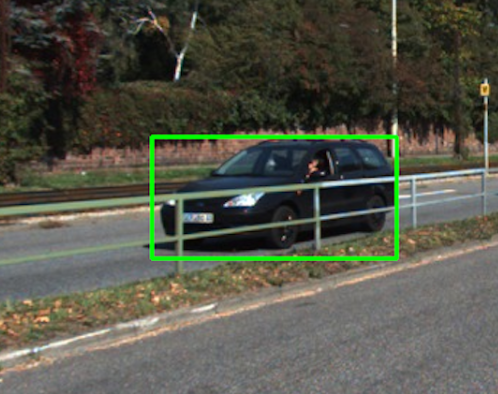
\includegraphics[width=0.2\textwidth]{figures/method/ambiguous/ex5/rgb.png}
        &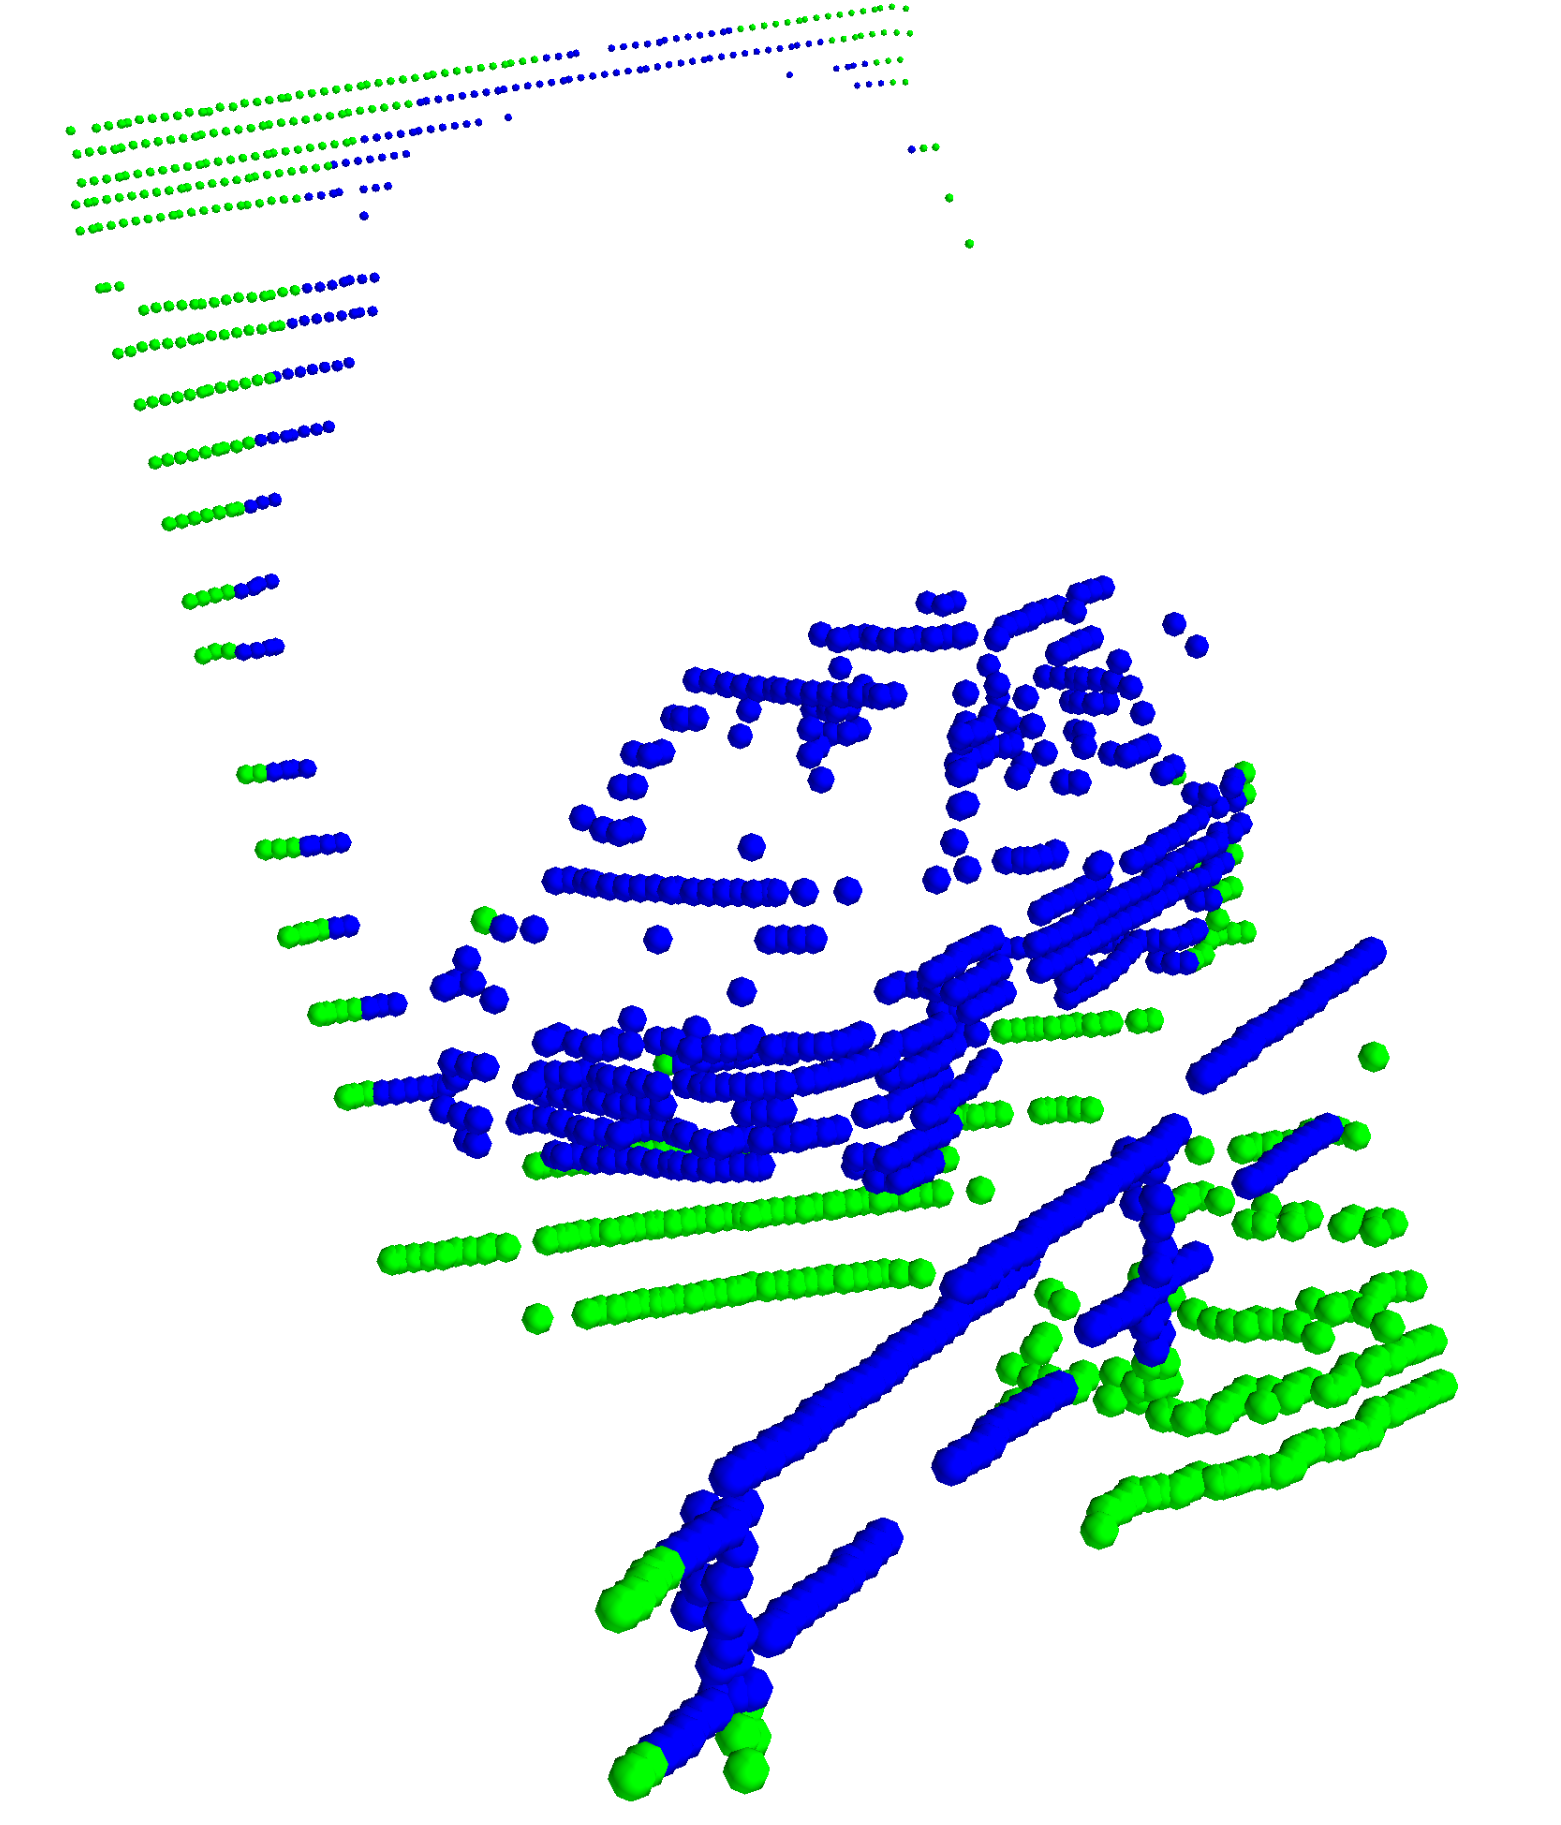
\includegraphics[width=0.2\textwidth]{figures/method/ambiguous/ex5/pcd.png}
        
    \end{tabular}
    
    \caption{Even with the pixel level Mask-RCNN detections our remaining pointclouds in blue can still have a lot of noise caused occluding objects or imperfect masks which cause problems for a chamfer distance like fit}
    \label{fig:dataset_example}
    
\end{figure}
\begin{figure}
    \centering
    
        
        \begin{tabular}{c c c c}
            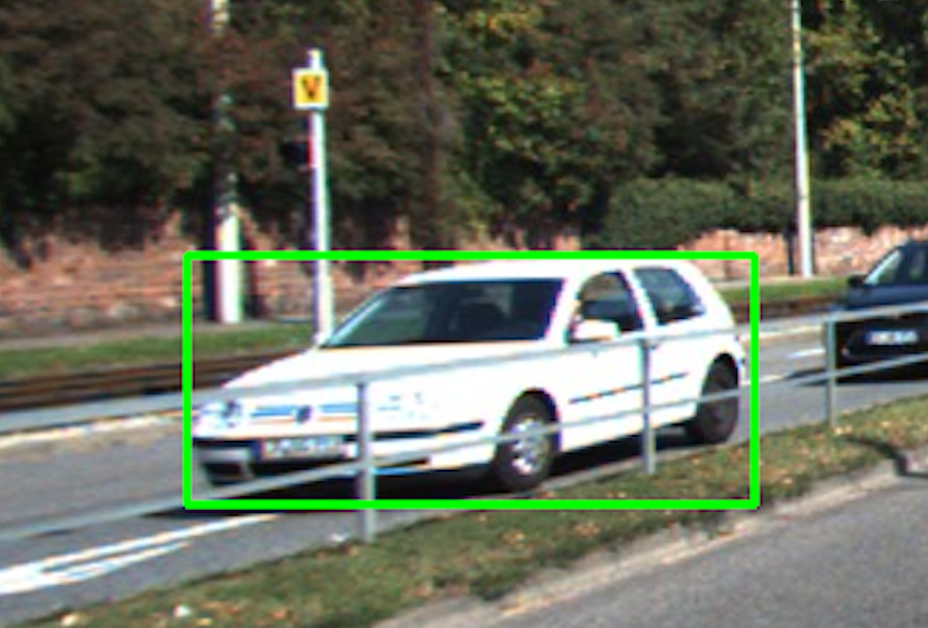
\includegraphics[width=0.25\textwidth]{figures/method/output_examples/rgb-1.png} &
            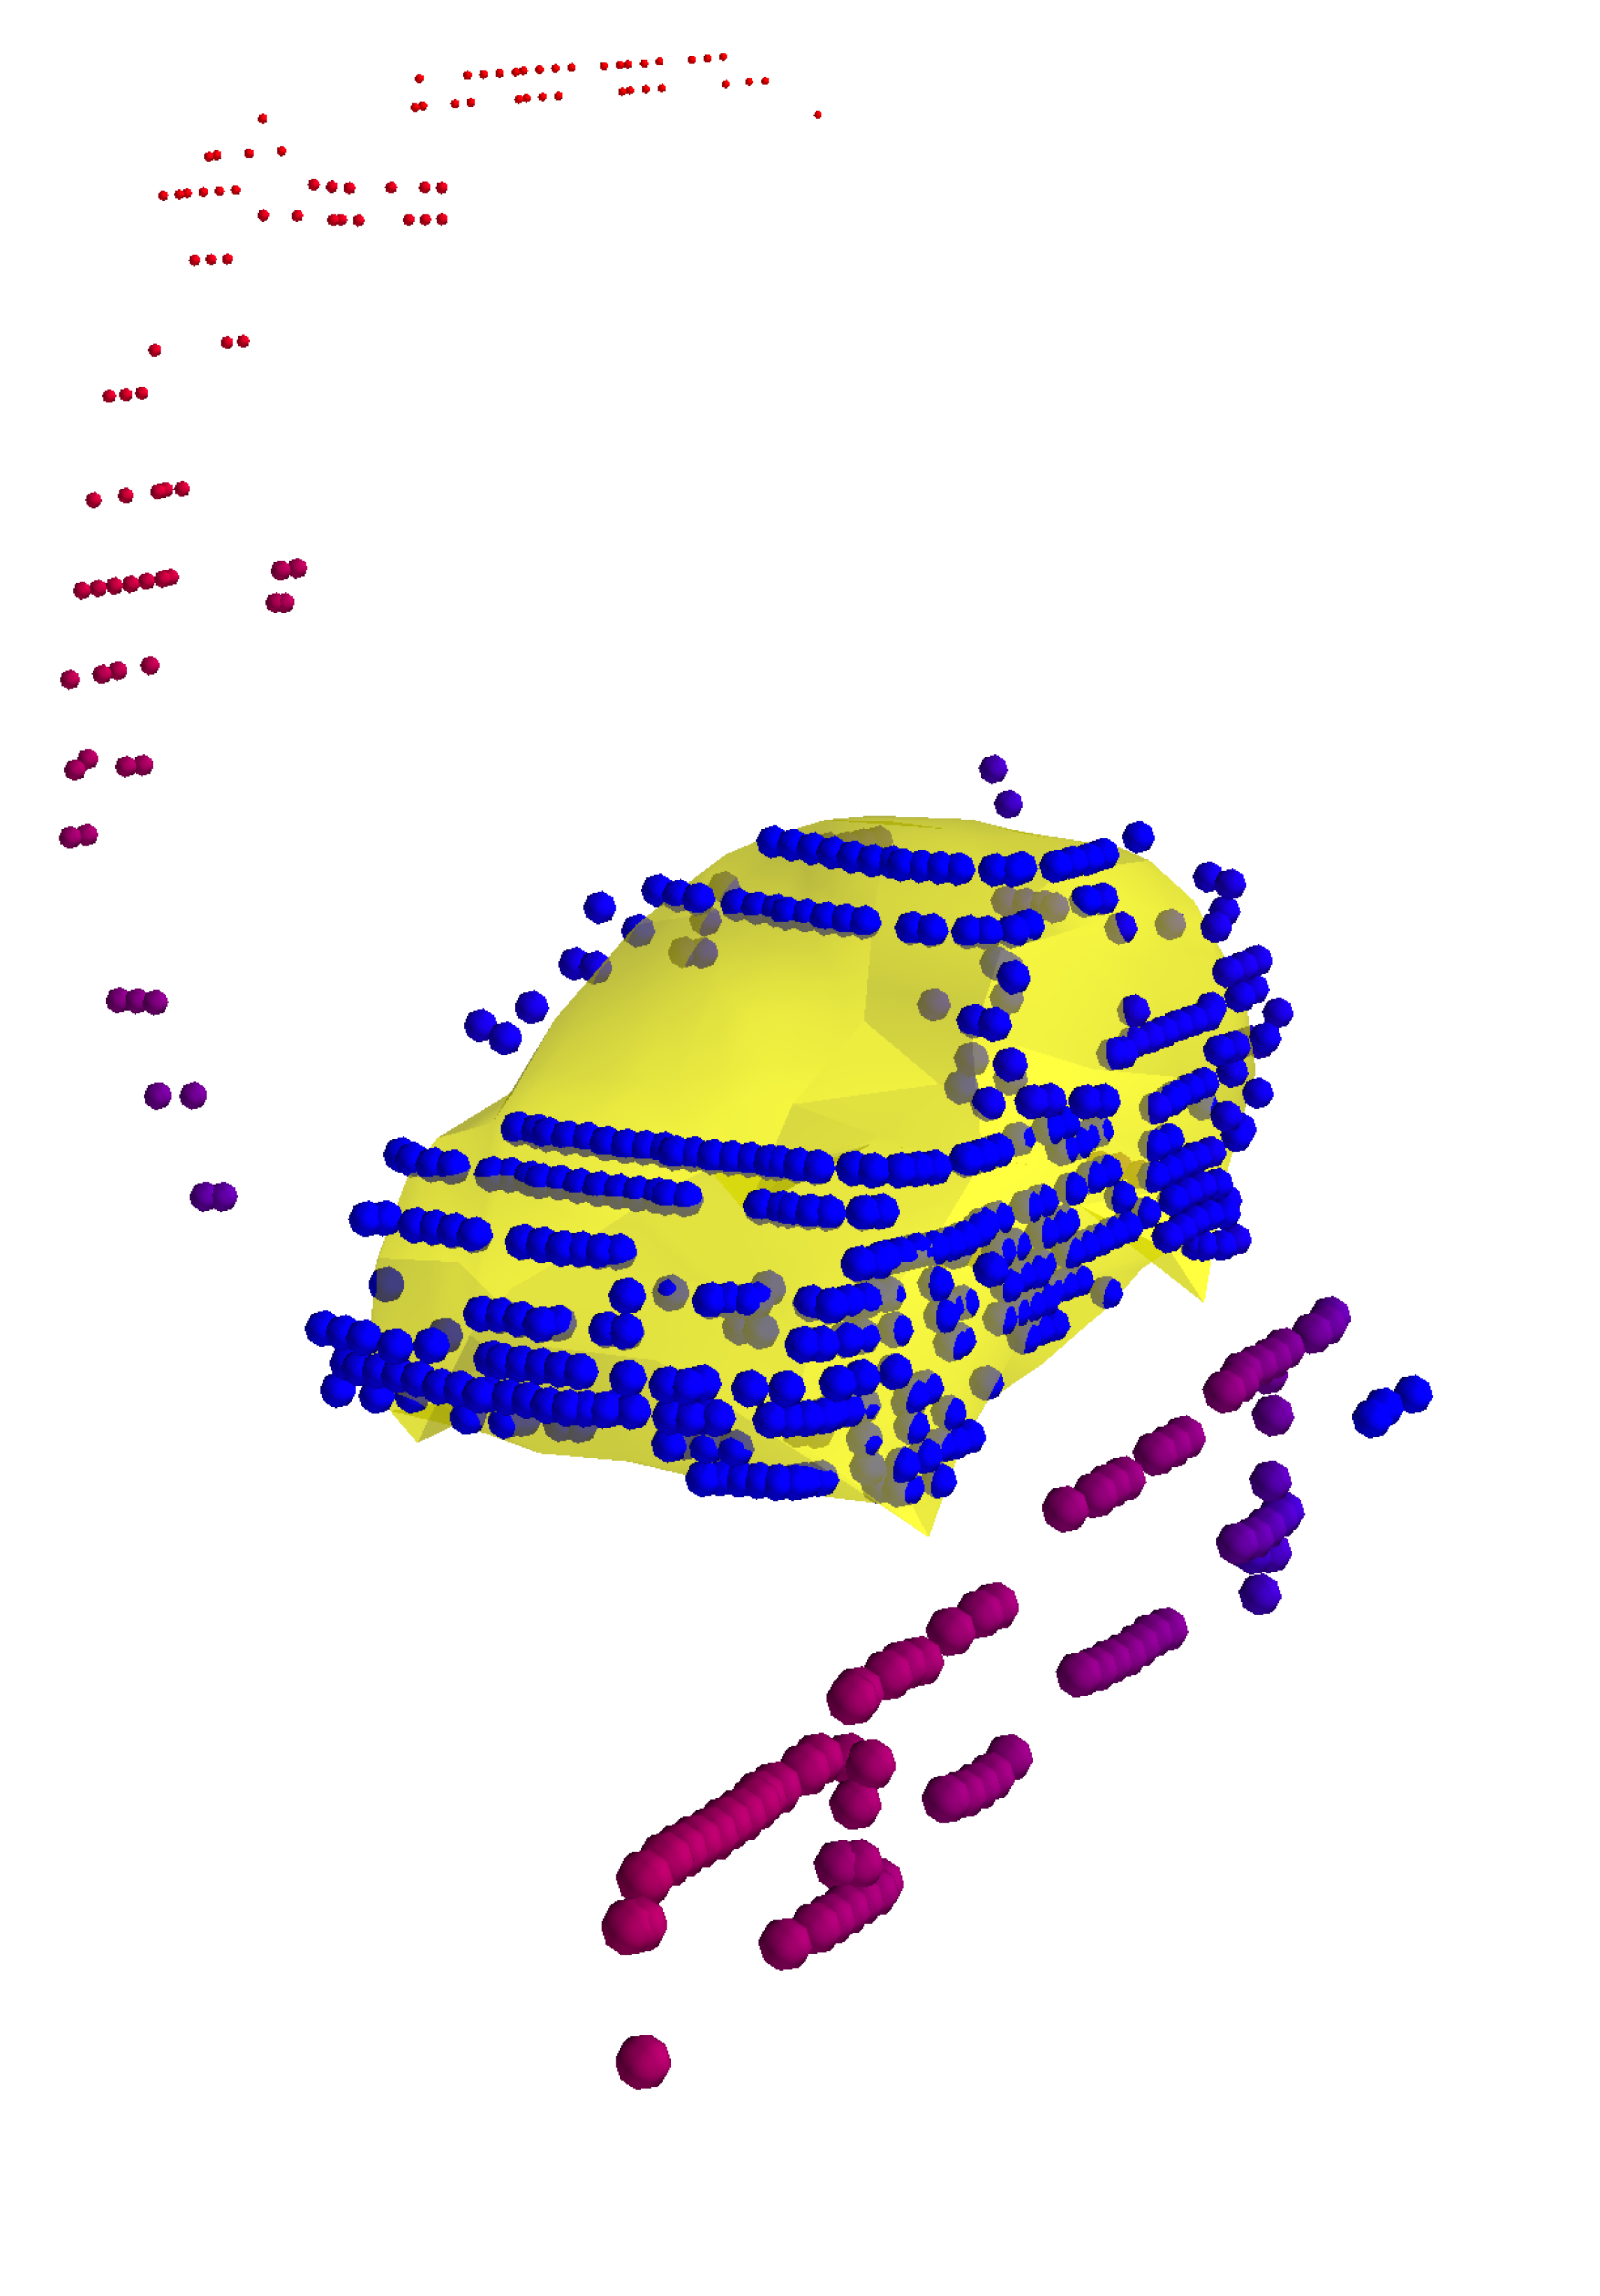
\includegraphics[width=0.25\textwidth]{figures/method/output_examples/pcd-1.png} &
            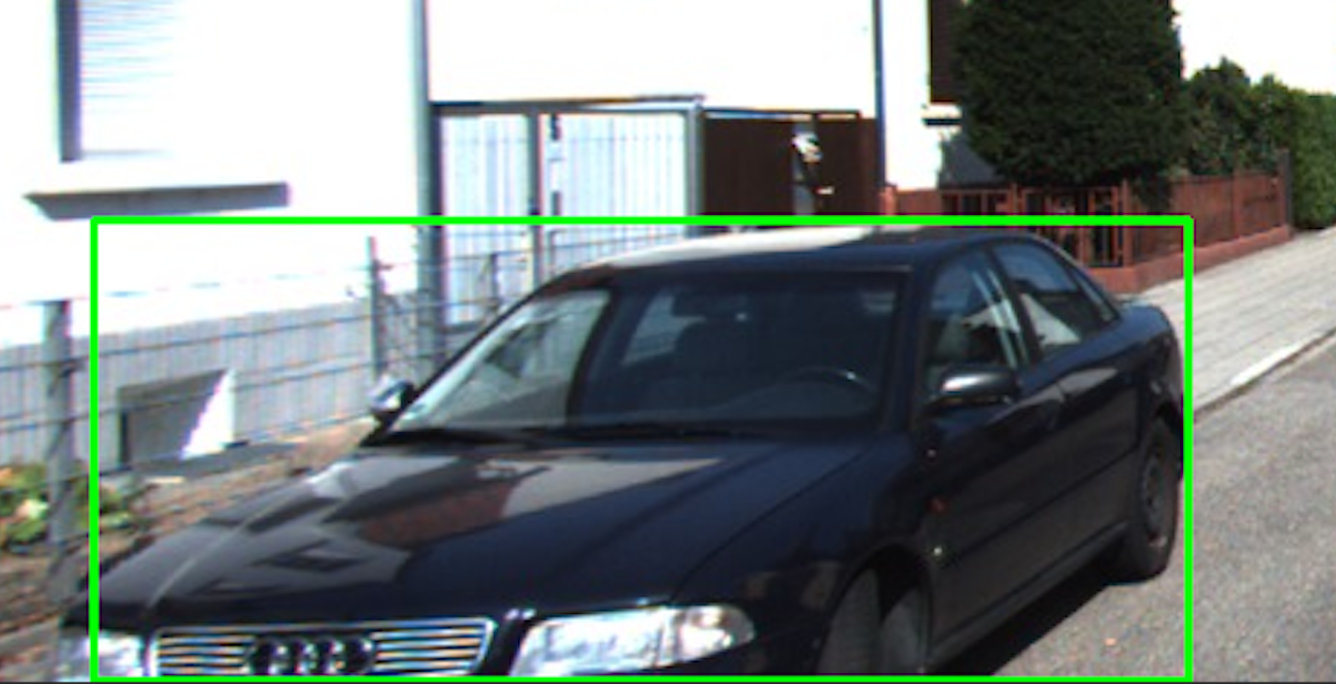
\includegraphics[width=0.25\textwidth]{figures/method/output_examples/rgb-2.png} &
            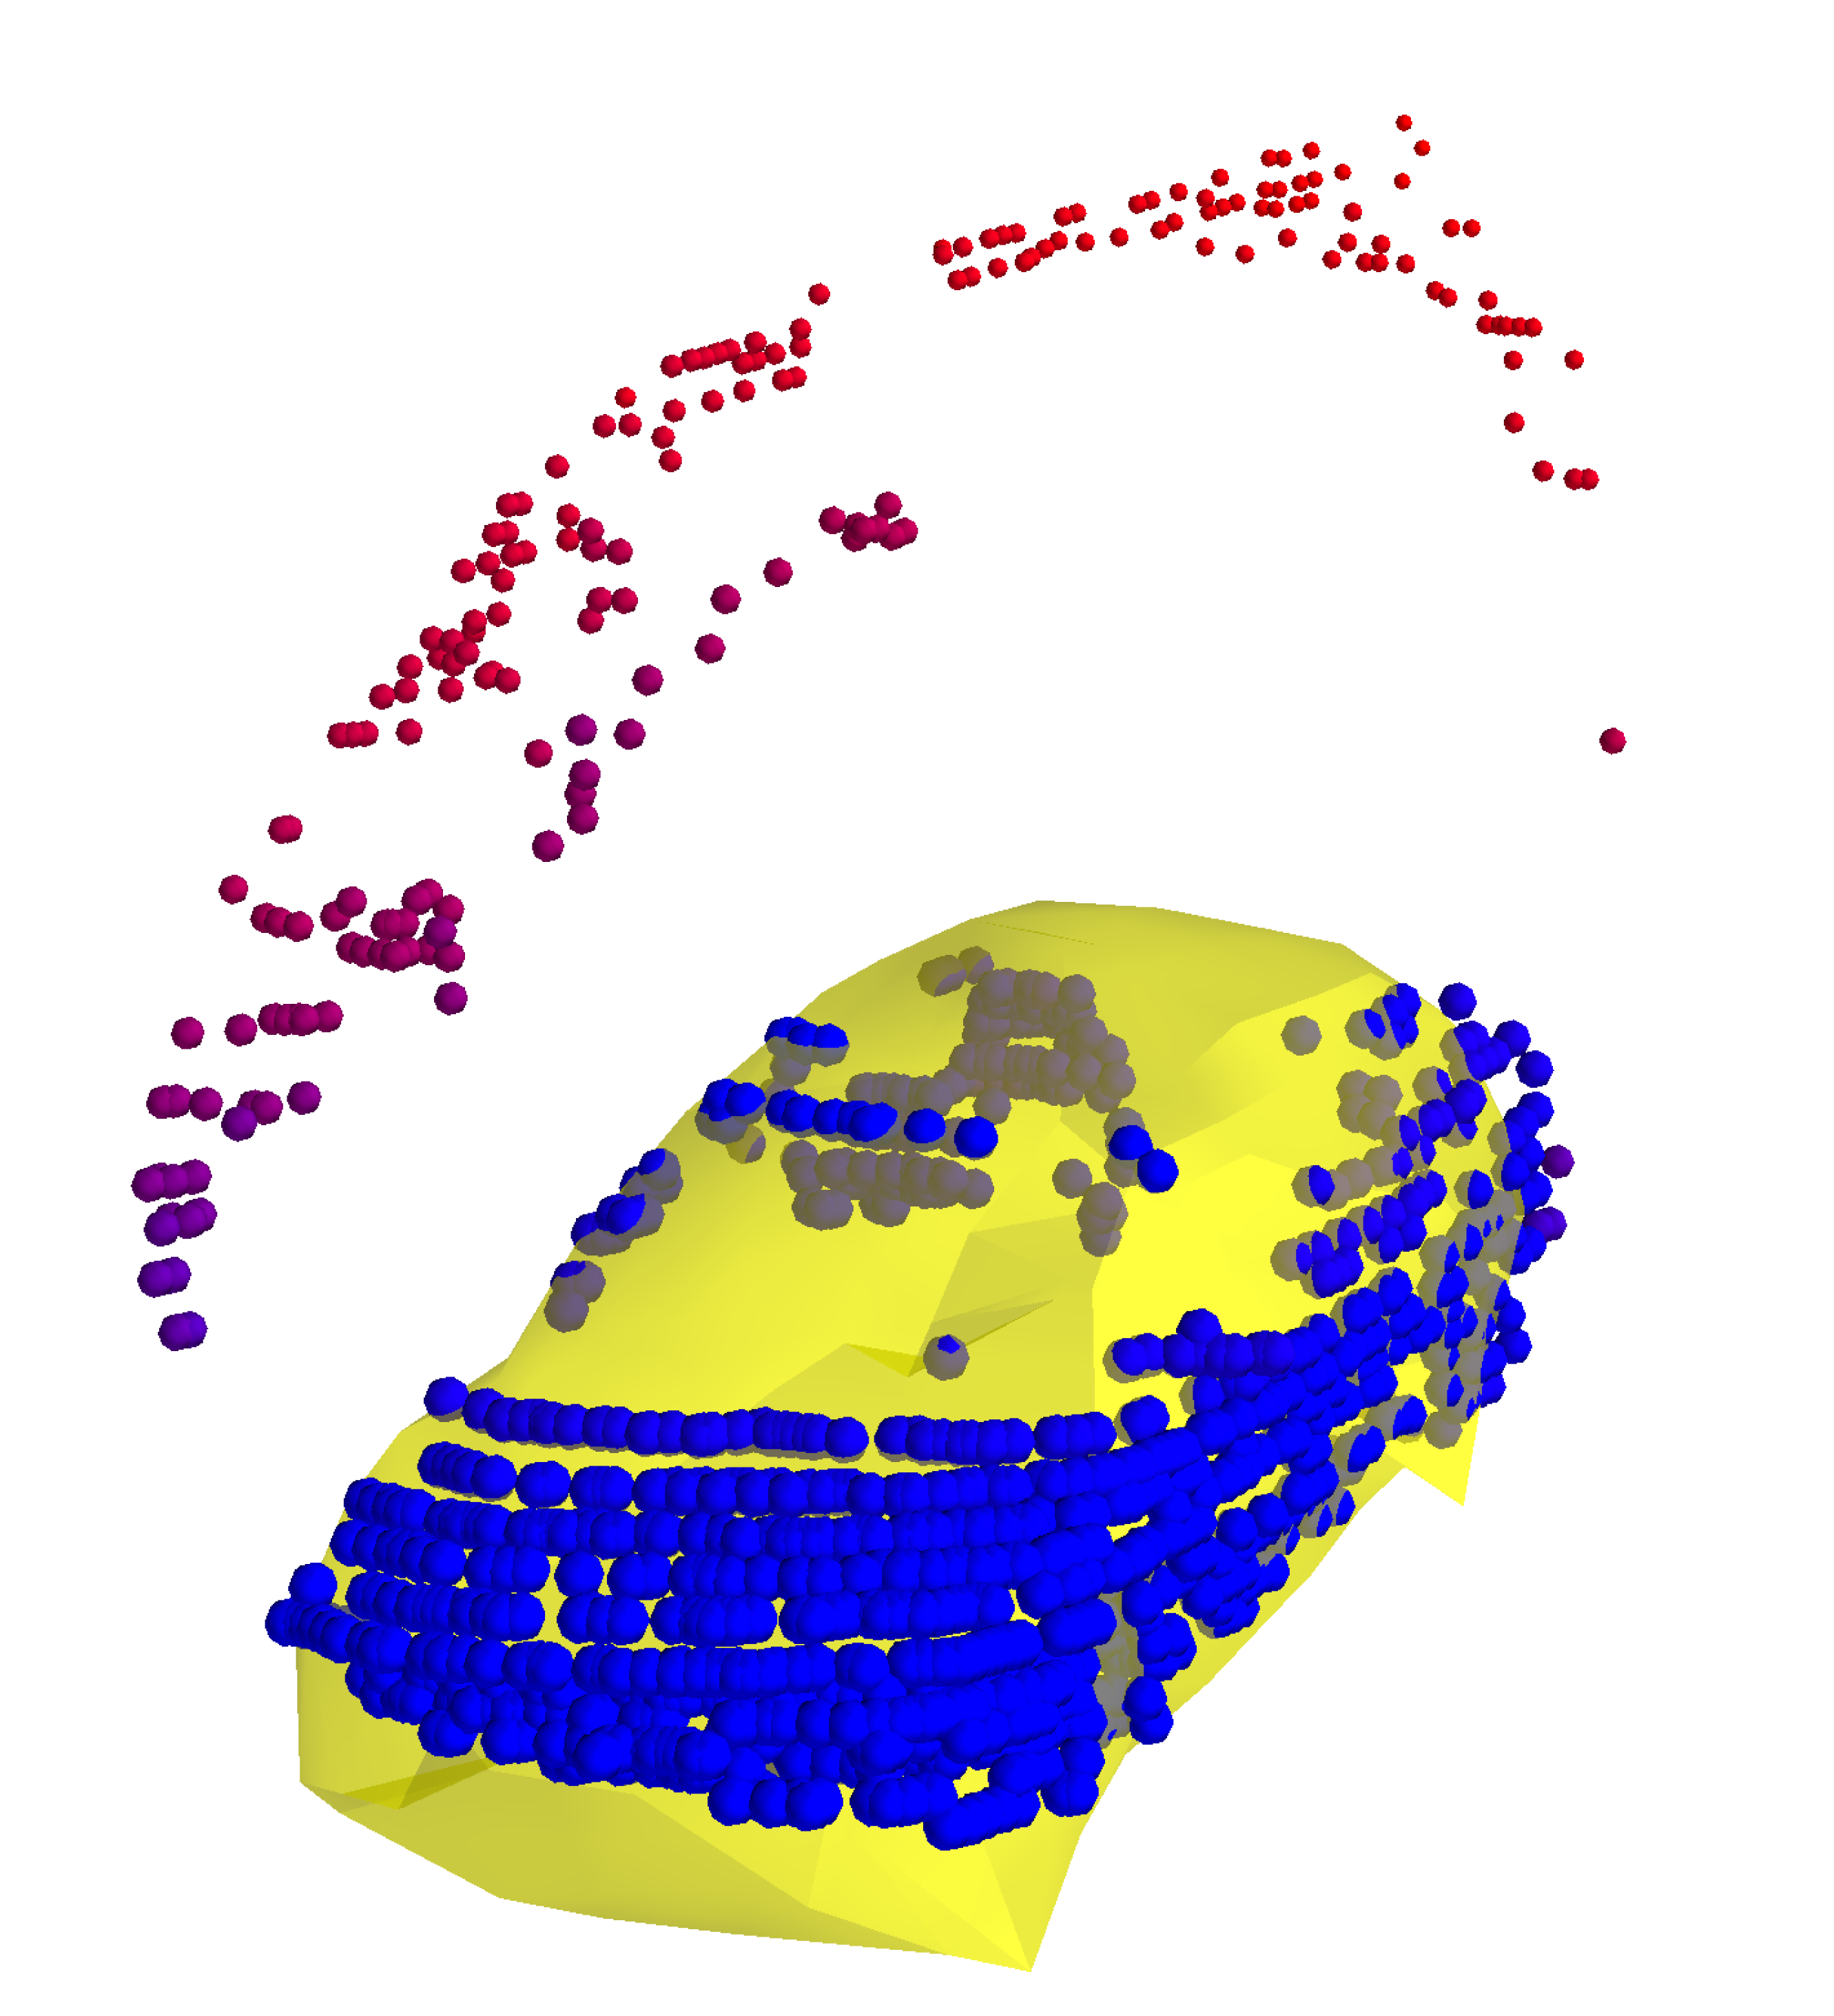
\includegraphics[width=0.25\textwidth]{figures/method/output_examples/pcd-2.png}
        \end{tabular}
        \caption{Even after removing LiDAR points which do not project into the 2D instance mask we still have a large number of outliers, mainly caused by partial occlusions and points at the boundary where 2D masks struggle. The $\sigma^2(\X)$ value predicts the relevance of a point to the cars location with blue points having low values with a gradient to red for higher values which suggests the point is an outlier.}
    \label{fig:my_label}
\end{figure}

A major drawback of~\cref{e:simpleloss} is that LiDAR points tend to be noisy, especially because the boundaries of the region $m$ may not correspond to the object exactly or the LiDAR may be affected by a reflection or `see through' a glass surface.
Such points might disproportionally skew the loss term, forcing the estimated object position closer to these outliers.
In order to help the model discriminate between inliers and outliers, we let the network predict an estimate of whether a given measurement is likely to belong to the object or not.

We therefore propose a second network $\sigma(\X) = \Psi_\X(L_m)$ that assigns to each LiDAR point $\X \in L_m$ a variance $\sigma$ and jointly optimize $\Phi$ and $\Psi$ by minimizing~\cite{novotny17learning,kendall17what}:
\begin{equation}\label{e:distance}
  \bar d(S|L_m)
  =
  %E_{\hat S}\left[
  \frac{1}{|L_m|}
  \sum_{\X \in L_m}
  \min_{\X' \in \hat S}
  \frac{\|\X' - \X \|^2}{\sigma^2(\X)}
  +
  \log \sigma^2(\X)
  %\right]
  % \label{e:sigmaloss}
  %  \mathcal{L}''(\Phi, \Psi|\mathcal{D})
  % &=
  % \frac{1}{|\mathcal{D}|}
  % \sum_{(L_m,m)\in\mathcal{D}}
  % \bar d(g_m S_0 | L_{m}).
\end{equation}
Note that the network $\Psi$ has to make a judgement call for every point $\X$ on whether it is likely to be an outlier or not \emph{without} having access to the loss.
A perfect prediction (i.e., one that minimizes the loss) would set $\sigma(\X) = \|\X' - \X \|$ to be the same as the fitting error.
The desirable side effect is that, in this manner, outliers are discounted by a large $\sigma(\X)$ when it comes to estimating the pose $g_m$ of the object.

% {\color{red}In practice, networks $(\Phi,\Psi)$ are implemented by branching off the same PointNet backbone, for computational and statistical efficiency (parameter sharing).  This is not the case at the minute but I want to try it}

\subsection{Direct optimization for the yaw}\label{s:direct-yaw}
% {\color{red} This title sounds like we have a learnable parmeter for yaw, perhaps "Hypothesis Testing for Yaw Estimation" }
\begin{figure}
    \centering
    \begin{tabular}{c c c c}
         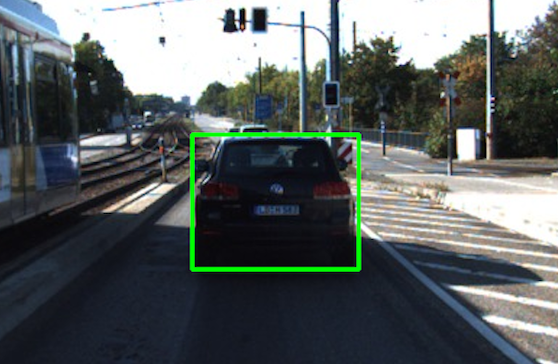
\includegraphics[height=0.135\textwidth]{figures/method/ambiguous/ex4/rgb.png}
        &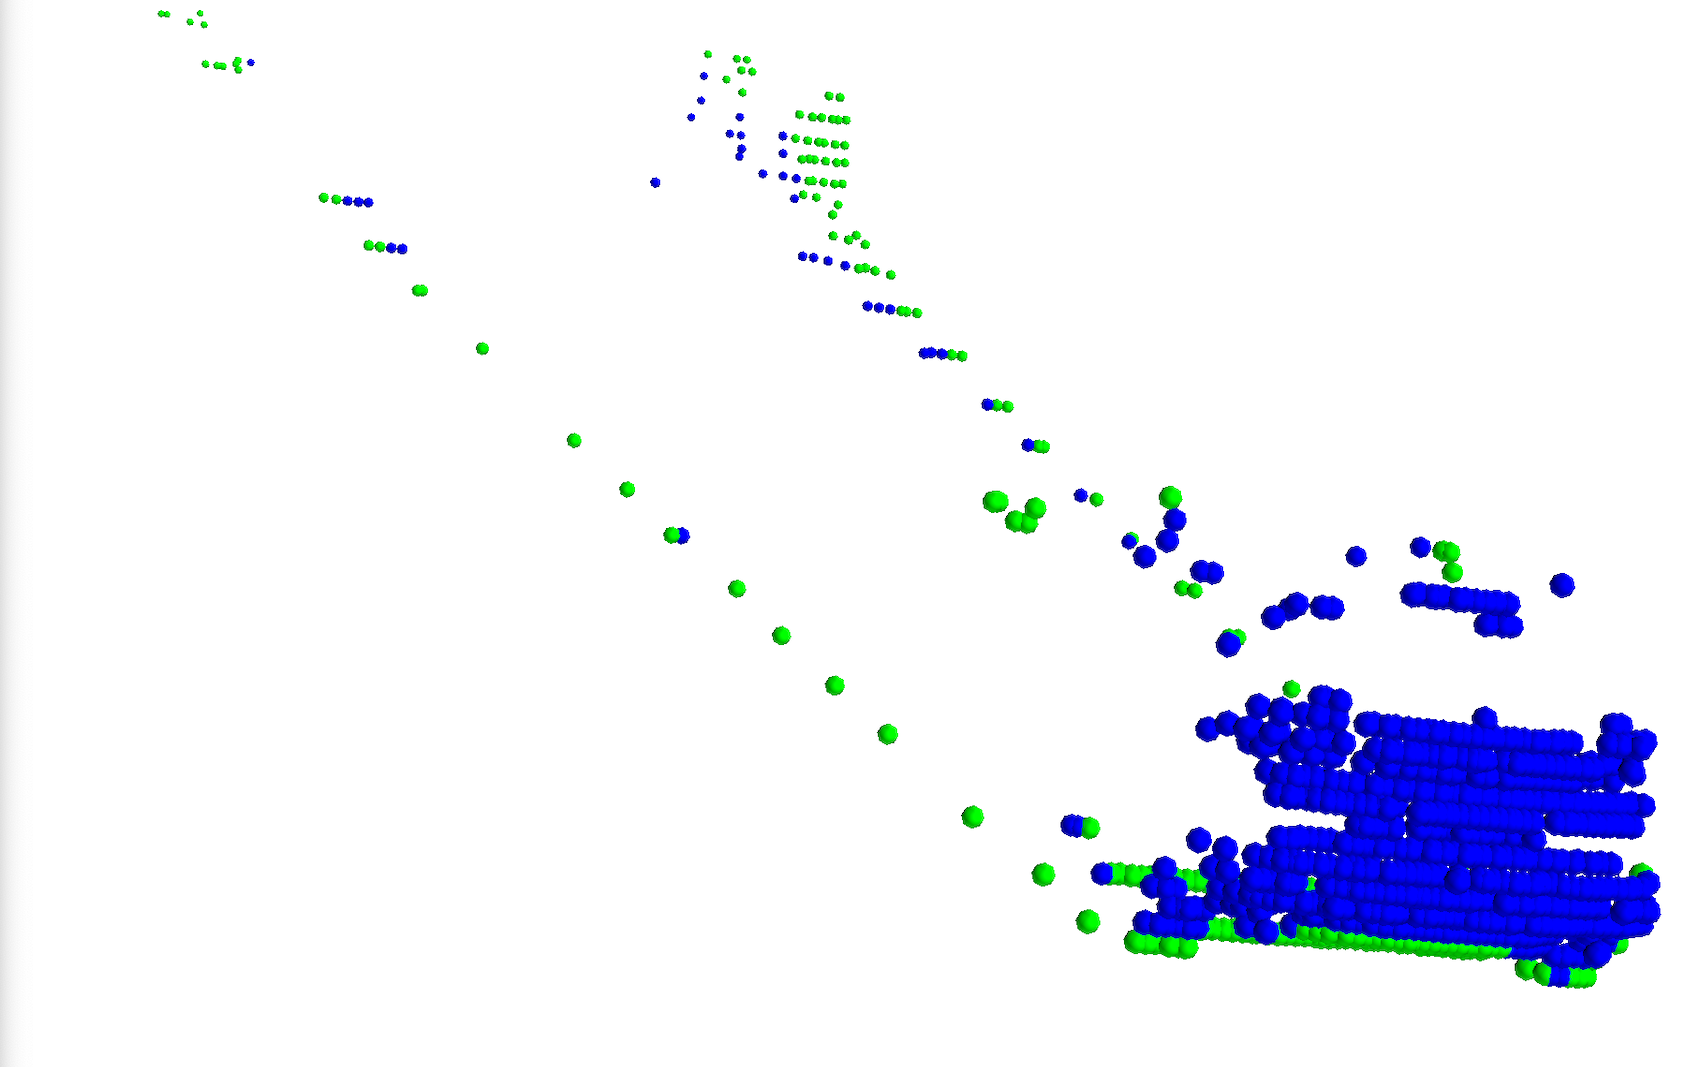
\includegraphics[height=0.135\textwidth]{figures/method/ambiguous/ex4/pcd.png} &
         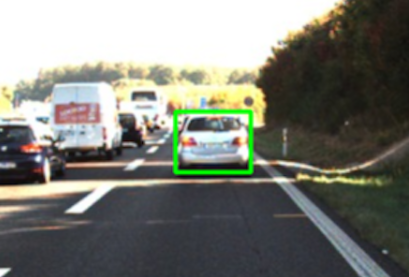
\includegraphics[height=0.135\textwidth]{figures/method/ambiguous/ex6/rgb.png}
        &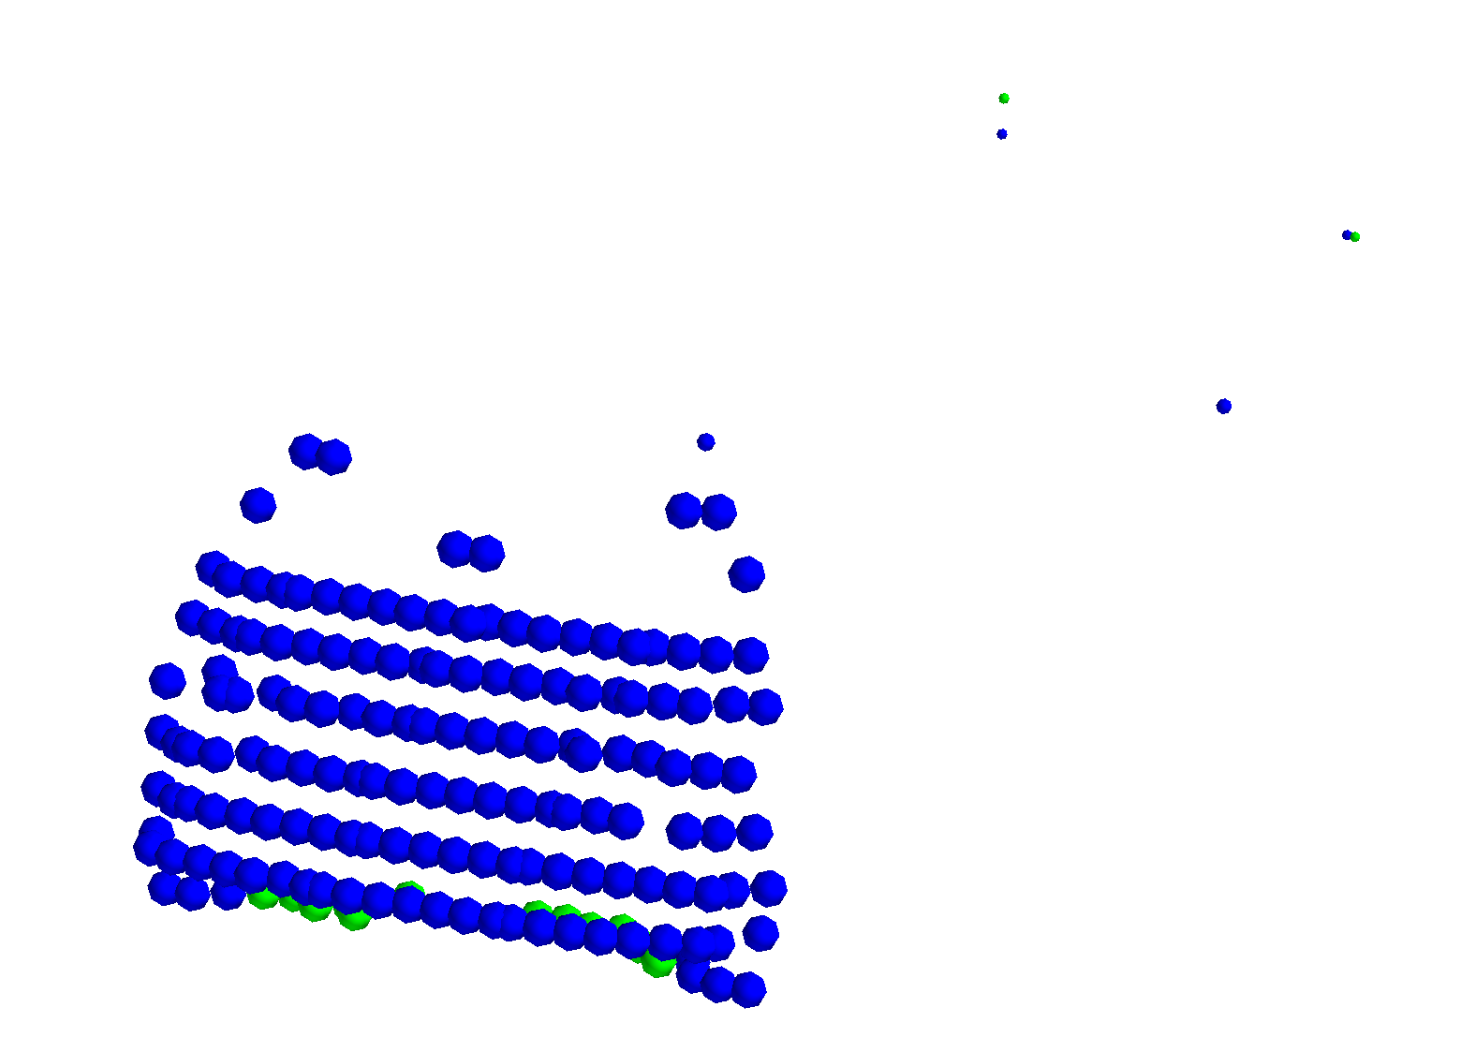
\includegraphics[height=0.135\textwidth]{figures/method/ambiguous/ex6/pcd.png}
    \end{tabular}
    \caption{In some cases the LiDAR point cloud only captures a single surface of the vehicle. This is problematic as fitting such point clouds is ambiguous, particularly for the rotation component.}\label{fig:ambiguous}
\end{figure}

Finally, we note that fitting the rotation of the object can be ambiguous, especially if only a small fragment of the object is visible in the RGB/LiDAR data.
Specifically, the distance $\bar d([R_{\theta_m}~\mathbf{T}_m]S_0|L_m)$, which is usually well behaved for the translation component $\mathbf{T}_m$, has instead a number of `deep' local minima, which we found is mainly caused by the inherent ambiguities of fitting the rotation $\mathbf{\theta}_m$ (yaw) parameter.
Specifically, each minimum corresponds to a $90^{\circ}$ rotation (see \cref{fig:ambiguous}).
In practice, as we show, the yaw network $\Psi$ \emph{can} learn to disambiguate the prediction, but it usually fails to converge to such a desirable solution without changes in the formulation.
% This ambiguity cannot be resolved from a single view, especially if only two or even one side of the car is visible - in this case the loss cannot distinguish whether front or back side of the car is captured.

In order to solve this issue, we propose to modify the formulation to incorporate \emph{direct optimisation} over the yaw.
In other words, every time the loss is evaluated, we assess a number of possible rotations $R$, as follows:
%
% In order to overcome these inherent ambiguities and the resulting local minima of the loss function during training, we propose a new training scheme which explicitly enumerates possible values of $\mathbf{R}_\theta$ from the set of possible values $\mathcal{R}$ in every training step, ensuring the optimizer never gets stuck in a local optimum
%
\begin{align}
  R^*_m
  &= \operatornamewithlimits{argmin}_{R\in \mathcal{R}}
  \bar d([R ~~\mathbf{T}_m] S_0 | L_{m})
  \\\label{e:iteratedloss}
  \mathcal{L}'(\Phi, \Psi|\mathcal{D})
  &=
  \frac{1}{|\mathcal{D}|}
  \sum_{(L_m,m)\in\mathcal{D}}
  \bar d([R^*_m~ \mathbf{T}_m] S_0 | L_{m}) + \lVert R_m - R_m^*\rVert .
\end{align}

The loss is the same as before for the translation, but, given the predicted translation, it always explores all possible rotations $R$, picking the best one $R_m^*$.

Note that this does not mean that the network $\Phi$ is not tasked with predicting a rotation anymore; on the contrary, the network is encouraged to output the optimal $R_m^*$ via minimization of the term $\|R_m - R_m^*\|$.
This has the obvious benefit of not incurring the search at test time, and therefore the final network running time is not affected by this process.

In practice, as only the yaw angle is predicted, we implement this loss by quantizing the interval $[0, 2\pi)$ in 64 distinct values (bins), as in our experiments we found this number of bins sufficient (see results in \cref{t:yaw}).
In this manner, the rotation head of the network $\Phi$ can be interpreted as a softmax distribution $\Phi_r(L_m)$ and the norm $\lVert . \rVert$ is replaced by the cross-entropy loss.

% $\hat{d}$ works quite well for centre estimation as the model $S_0$ must be minimally distant to the LiDAR points $L_m$. Yaw on the other hand is a more difficult parameter to estimate as there is an inherent discontinuity at the end of the range of possible values. This can be approached numerous ways, some have approached yaw as a vector prediction task where the vector is converted to a yaw using the arctan function, quaternions are used similarly. Others utilise quantised bins which are predicted using a cross entropy loss.\\
% Predicting Yaw as one of $n$ quantised steps is well studied approach in supervised learning approaches. Compared to continuous predicted values in the vector and quaternion approaches this does not have an issue with the discontinuity present at the jump between $0$ and $2\pi$ where the the loss value is quite high but the actual error is relatively quite small. To train our model to predict the correct yaw bin without supervision we need to determine the correct bin for our input pointcloud $L_m$. We achieve this by transforming our reference model $S_0$ by the centre predicted by $\Phi$ and rotating by each of the bins yaws. This ensemble of yaws is then ranked by applying $\hat{d}$ to each of them and picking the hypothesis with minimal loss.
% \begin{equation}
%     \amin_{y\in \{\frac{i2\pi}{b} | i\in[0...b-1]\}} \hat{d}(\bold{R}(y,XYZ)|L_m)
% \end{equation}
% where $\bold{R}(y,XYZ)$ is the transformation matrix generated by the candidate yaw $y$ and the centre prediction $XYZ$. This minimum is expensive to compute as is requires running $\hat{d}$ $b$ times per forward pass. Instead performing this at test time we use the index of the bin which resulted in minimal error to train a subnetwork of the RT network to predict the yaw bin which is minimal.

\subsection{Multi-frame consistency}

\begin{figure}
    \centering
    \begin{tabular}{c c | c c}
        \multicolumn{2}{c}{Frame 1} & \multicolumn{2}{c}{Frame 5} \\
        %\hline
        %  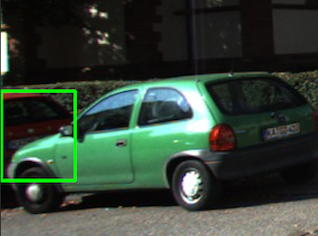
\includegraphics[width=0.2\textwidth]{figures/method/multiframe/ex1/rgb-1.png}
        % &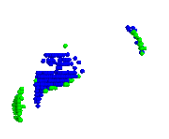
\includegraphics[width=0.2\textwidth]{figures/method/multiframe/ex1/pcd-1.png} &
        %  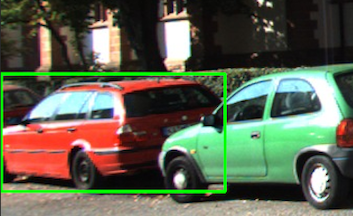
\includegraphics[width=0.2\textwidth]{figures/method/multiframe/ex1/rgb-5.png}
        % &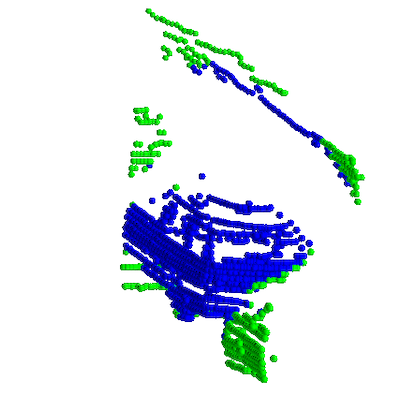
\includegraphics[width=0.2\textwidth]{figures/method/multiframe/ex1/pcd-5-1.png} \\
         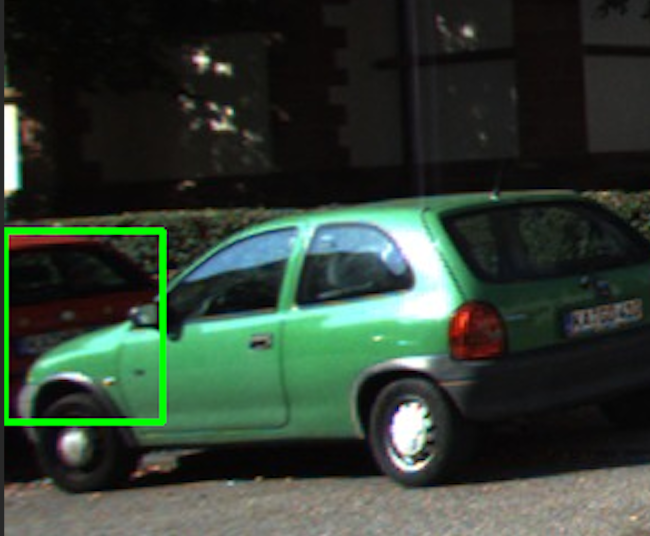
\includegraphics[height=0.16\textwidth]{figures/method/multiframe/ex3/rgb-1.png}
        &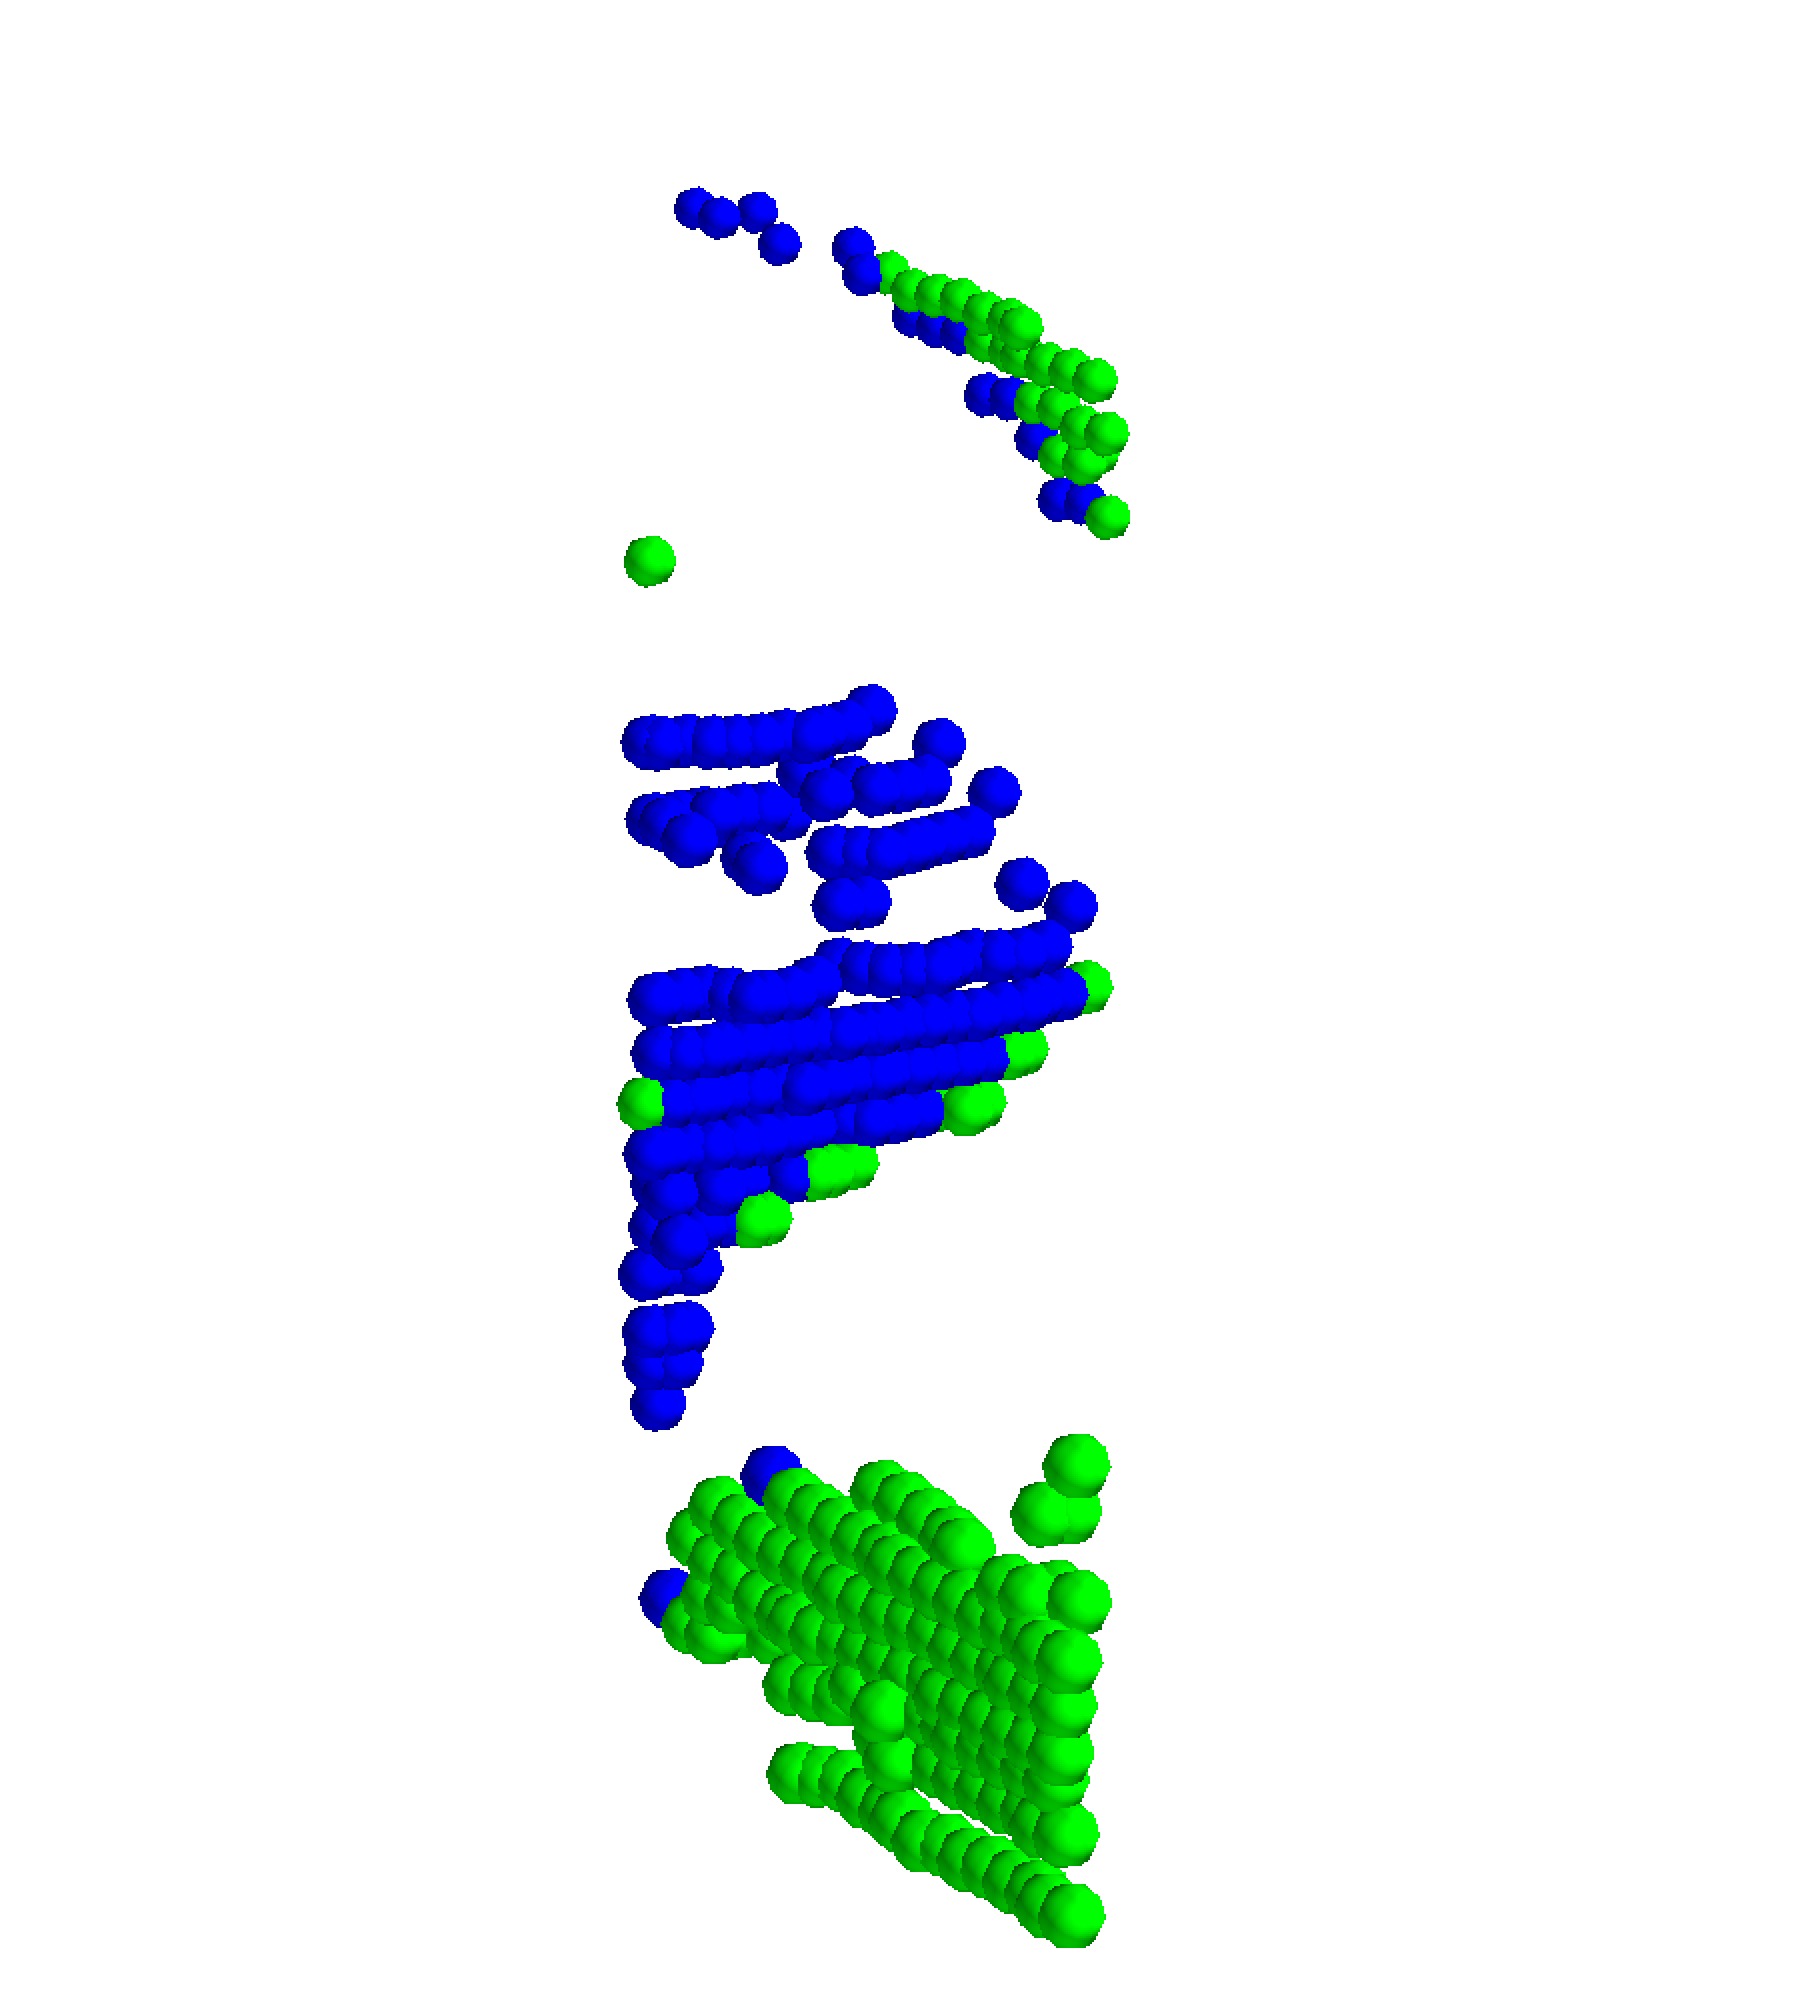
\includegraphics[width=0.15\textwidth]{figures/method/multiframe/ex3/pcd-1.png} &
         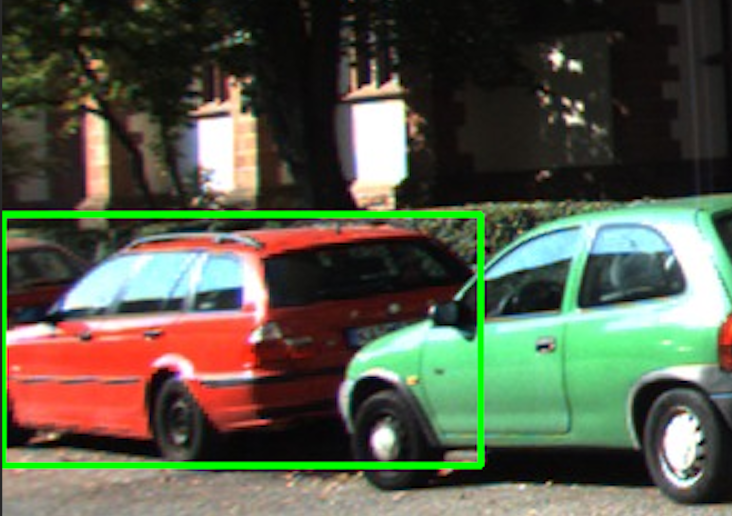
\includegraphics[height=0.16\textwidth]{figures/method/multiframe/ex3/rgb-5.png}
        &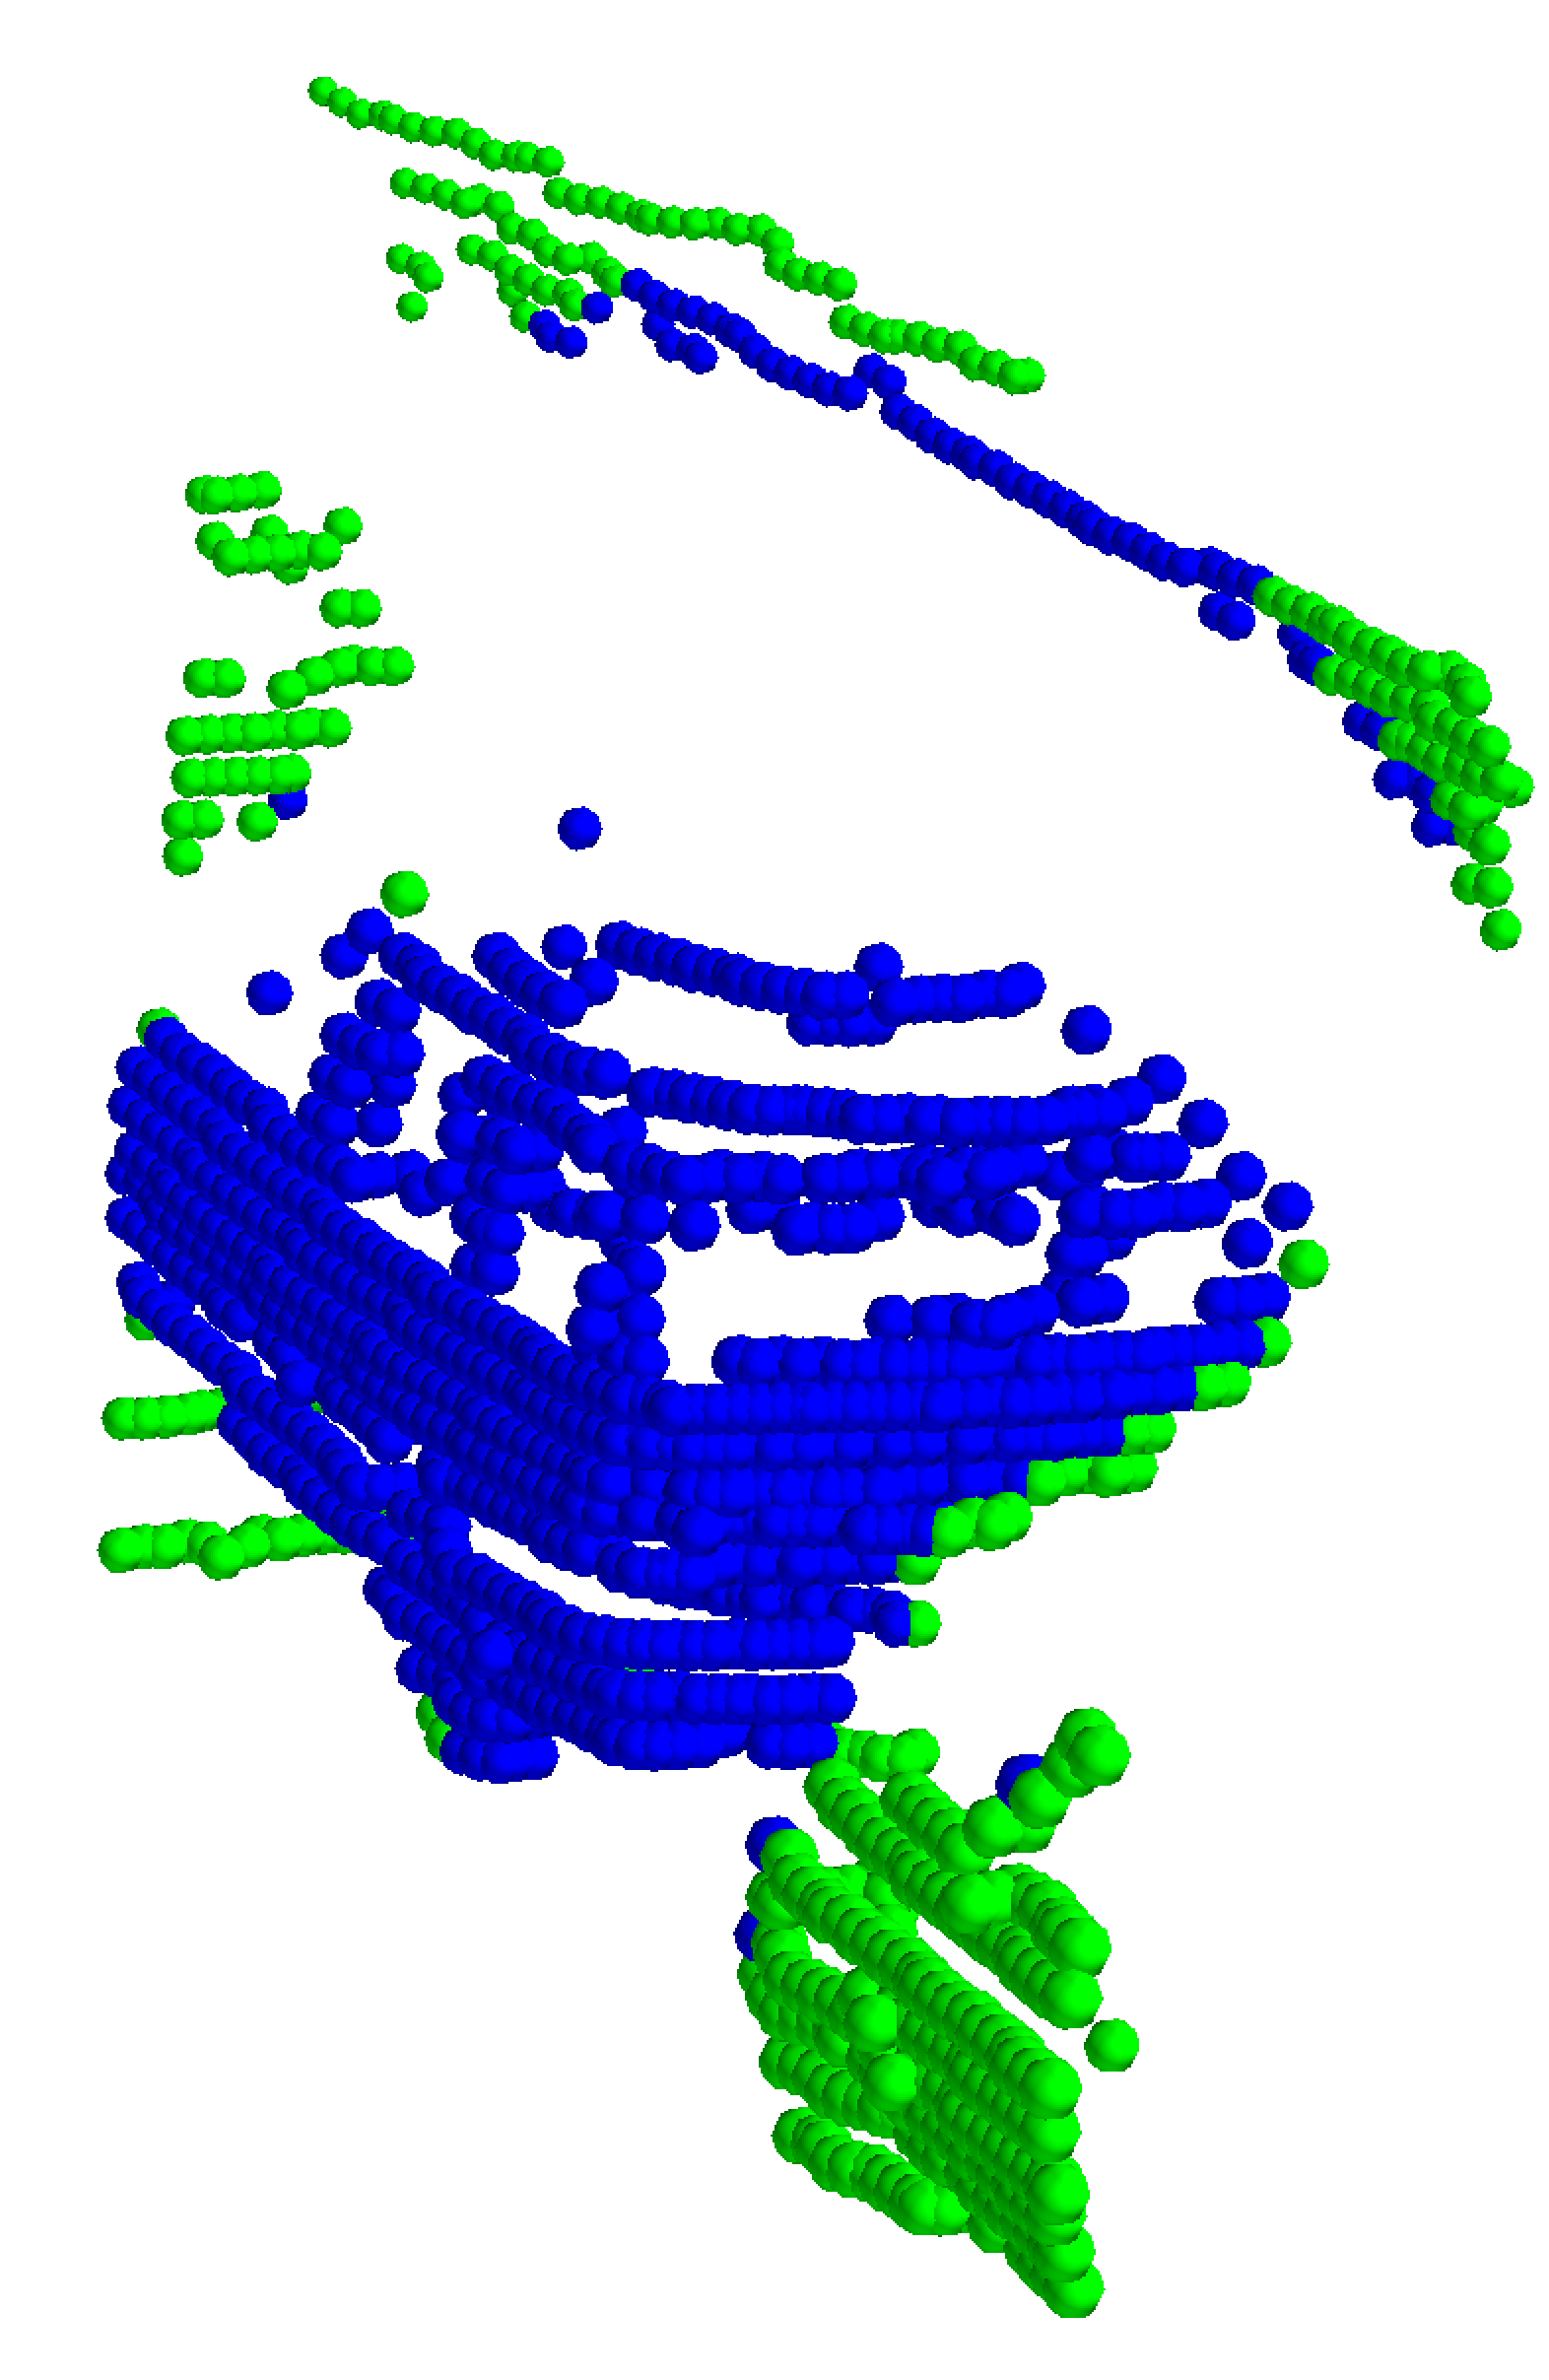
\includegraphics[height=0.2\textwidth]{figures/method/multiframe/ex3/pcd-5.png} \\
    \end{tabular}
    \caption{Two frames in a sequence of five, with a heavily occluded and truncated car in the first frame and a much better view of the same in the last.
    Multi-frame consistency allows the method to use clearer frames to interpret more difficult ones, which is particularly helpful in discovering the outliers.}\label{fig:multiframe_example}
    % On the left we see examples from the first frame of five where the car of interest is heavily occluded or truncated.
    % whereas in the last frame the vehicle is much better described by the point cloud allowing our method to more confidently fit and thus improve the difficult examples through consistency}
\end{figure}

Whilst in our approach we do not have the actual 3D pose of the object available as a training signal, the 3D pose of the object across multiple frames must be consistent with the observer ego-motion.
This is true for vehicles that are not moving (parked cars) and approximately true for other vehicles; in particular, the \emph{yaw} of the objects, once ego-motion has been compensated for, is roughly constant.

% it is still possible to use the equivarinace of the (unknown) 3D pose across multiple frames with respect to the ego-vehicle motion  as an additional training objective.

% Specifically, consider an arbitrary world point $\X^i\in\mathbb{R}^3$ observed in a LiDAR frame $j$.
% The position of the same point in a frame $i$ is given by
% \begin{align}
%     \X^i &= g_{i \leftarrow j} \X^j
% \end{align}
% where $g_{i \leftarrow j}$ is the ego-motion between frames $i$ and $j$ of the vehicle where the sensors are mounted, assuming the absolute position of the world point does not change.

% We then define an additional loss term $\mathcal{L^\X}$ for a well-defined (key-)point $\X$ as

% \begin{align} \label{e:keypointloss}
%    \mathcal{L^\X}(\Phi, \Psi|\mathcal{D})
%   &=
%   \frac{1}{|\mathcal{D}|}
%   \sum^N_{i=1}
%   \sum_{(L_m,m)\in\mathcal{D}^i}
%   \sum^K_{j=1} \lVert\ \mathbf{P}_{i + j\rightarrow i}\X^{i+j}_m - \X^i_m\rVert^2
% \end{align}

Specifically, consider an arbitrary model point $\X_0\in S_0$.
Observed in a LiDAR frame $i$, this point is estimated to be at location $\X_0^i = g^i \X_0$, where $g^i$ is the network prediction for frame $i$.
Likewise, let $\X_0^j = g^j \X_0$ be the point position at frame $j$.
If the object is at rest, the two positions are related by
$
    \X^i_0 = g_{i \leftarrow j} \X^j_0
$
where $g_{i \leftarrow j}$ is the ego-motion between frames $i$ and $j$ of the vehicle where the sensors are mounted, which we assume to be known.
We can thus define the consistency loss $\mathcal{L}^{\X_0}$ for any model point $\X_0$:
%
\begin{equation}\label{e:keypointloss}
   \mathcal{L}^{\X_0}(\Phi|\mathcal{D})
=
  \frac{1}{|\mathcal{D}|}
  \sum^N_{i=1}
  \sum_{(L_m,m)\in\mathcal{D}^i}
  \sum^K_{j=1} \lVert\ g_{i \leftarrow i + j}
  \X_0^{i+j} - \X_0^i
  \rVert^2.
\end{equation}
where $\mathcal{D}^i$ denotes LiDAR-mask pairs detected in the frame $i$, $K$ is the length of the frame sequence over which the consistency is evaluated, and $N$ is the total number of frames.

Note that loss~\eqref{e:keypointloss} is null for all object keypoints if, and ony if, $g^i = g_{i\leftarrow j}g^j$, which is an \emph{equivariance} condition for the predictor.
However, we found it more convenient and robust to enforce this equivariance by using~\cref{e:keypointloss} summed over a small set of representative model points.
% More precisely, we choose specific points of the shape model (defined in \cref{s:shapemodel}), but because our shape model is rigid the choice can be fairly arbitrary.
In our experiments we have found that at least two points are required to ensure that we consistently predict the heading (yaw) of the detected car.
In practice, we use car centre and front keypoints (see \cref{f:Qualitative}), so the final loss term used to train the model is:
\begin{equation}\label{e:finalloss}
\mathcal{L}(\Phi, \Psi|\mathcal{D}) =
\mathcal{L}'(\Phi,\Psi|\mathcal{D})
+ \mathcal{L}^{\X_\text{center}}(\Phi|\mathcal{D})
+ \mathcal{L}^{\X_\text{front}}(\Phi|\mathcal{D})
\end{equation}

\paragraph{Implementation details: tracking.}

A detector such as Mask R-CNN only provides 2D mask for individual video frames, but defining the loss~\eqref{e:keypointloss} requires to identify or track the same object across two frames.
For tracking, we take the median of LiDAR points for each mask and compare them to the medians of masks in adjacent frames.
The closest pseudo-centres are chosen to be the same vehicle if and only if the number of LiDAR points has not changed significantly and the distance between them is less than 2 meters when ego motion is accounted for.
The distance criterion ensures that the same vehicle is detected while the number of points removes poor Mask-RCNN detections in subsequent frames.

